%% This file is cloned from `sample-sigconf.tex',
\documentclass[sigconf]{acmart}
%% BibTeX command to typeset BibTeX logo in the docs
\AtBeginDocument{%
  \providecommand\BibTeX{{%
    Bib\TeX}}}
\setcopyright{acmlicensed}
\copyrightyear{2024}
\acmYear{2024}
\acmDOI{XXXXXXX.XXXXXXX}
\acmConference[EuroPLoP '24]{29th European Conference on Pattern Languages of Programs}{July 3--7, 2024}{Kloster Irsee, Germany}
\acmISBN{978-1-4503-XXXX-X/18/06}
% ============================================================
% https://www.europlop.net
%    FEBRUARY 5, 2024 - Deadline for initial paper submission
%    MARCH 10, 2024 -  Acceptance for shepherding; Start of shepherding
%    JUNE 16, 2024 - End of shepherding; Deadline for conference version of paper
% ============================================================
% ============================================================
\usepackage{xspace}
\usepackage{graphicx}
\graphicspath{{figures/}}
% ============================================================
%% Uncomment the next few lines to get sf url links:
%\usepackage{url}            
%\makeatletter
%\def\url@leostyle{%
%  \@ifundefined{selectfont}{\def\UrlFont{\sf}}{\def\UrlFont{\small\sffamily}}}
%\makeatother
%\urlstyle{leo} % Now actually use the newly defined style.
%% Choose coloured or b/w links:
%\usepackage[pdftex,colorlinks=true,pdfstartview=FitV,
% linkcolor=black,citecolor=black,urlcolor=black]{hyperref}
%\usepackage{hyperref}
\usepackage{needspace}
\newcommand{\needlines}[1]{\Needspace{#1\baselineskip}}
\usepackage{paralist}
% ============================================================
%:Markup macros for proof-reading
\usepackage{ifthen}
\usepackage[normalem]{ulem} % for \sout
\usepackage{xcolor}
\newcommand{\ra}{$\rightarrow$}
\newboolean{showedits}
\setboolean{showedits}{true} % toggle to show or hide edits
%\setboolean{showedits}{false} % toggle to show or hide edits
\ifthenelse{\boolean{showedits}}
{
	\newcommand{\meh}[1]{\textcolor{red}{\uwave{#1}}} % please rephrase
	\newcommand{\ins}[1]{\textcolor{blue}{\uline{#1}}} % please insert
	\newcommand{\del}[1]{\textcolor{red}{\sout{#1}}} % please delete
	\newcommand{\chg}[2]{\textcolor{red}{\sout{#1}}{\ra}\textcolor{blue}{\uline{#2}}} % please change
	\newcommand{\nbe}[3]{
		{\colorbox{#3}{\bfseries\sffamily\scriptsize\textcolor{white}{#1}}}
		{\textcolor{#3}{\sf\small$\blacktriangleright$\textit{#2}$\blacktriangleleft$}}}
}{
	\newcommand{\meh}[1]{#1} % please rephrase
	\newcommand{\ins}[1]{#1} % please insert
	\newcommand{\del}[1]{} % please delete
	\newcommand{\chg}[2]{#2}
	\newcommand{\nbe}[3]{}
}
%
\newcommand\rA[1]{\nbe{Reviewer A}{#1}{cyan}}
\newcommand\rB[1]{\nbe{Reviewer B}{#1}{olive}}
\newcommand\rC[1]{\nbe{Reviewer C}{#1}{magenta}}
\newcommand\ANS[1]{\nbe{Response}{#1}{teal}}

\newcommand{\THE}{\ins{the}\xspace} % "the" missing
\newcommand{\A}{\ins{a}\xspace} % "a" missing
\newcommand{\s}{\ins{s}\xspace} % "s" missing
\newcommand{\COMMA}{\ins{,}\xspace} % "," missing
\newcommand{\THAT}{\chg{which}{that}\xspace} % use "that", not "which"

% ============================================================
%:Box comments/edits
\usepackage[most]{tcolorbox}
\ifthenelse{\boolean{showedits}}
{
  \newtcolorbox{inserted}{%
       title=Inserted text:,
       colframe=blue,colback=blue!5!white,
       breakable,
       leftrule=0mm, 
       bottomrule=0mm,
       rightrule=0mm,
       toprule=0mm,
       arc=0mm, outer arc=0mm,
       oversize
  }
  \newtcolorbox{deleted}{%
       title=Deleted text:,
       colframe=red,colback=red!5!white,
       breakable,
       leftrule=0mm, 
       bottomrule=0mm,
       rightrule=0mm,
       toprule=0mm,
       arc=0mm, outer arc=0mm,
       oversize
  }
  \newtcolorbox{refactored}{%
       % title=Heavily modifed/refactored text:,
       title=Rewritten text:,
       colframe=blue,colback=red!5!white,
       breakable,
       leftrule=0mm, 
       bottomrule=0mm,
       rightrule=0mm,
       toprule=0mm,
       arc=0mm, outer arc=0mm,
       oversize
  }
}{
  \newenvironment{inserted}{}{}
  %\newenvironment{deleted}{ \begin{comment} }{ \end{comment} }
  \let\deleted\comment
  \newenvironment{refactored}{}{} 
}
% ============================================================
%:Put edit comments in a really ugly standout display
%\usepackage{ifthen}
%\usepackage{amssymb} % Avoid error: Command `\Bbbk' already defined.
\newboolean{showcomments}
\setboolean{showcomments}{true}
%\setboolean{showcomments}{false}
\newcommand{\id}[1]{$-$Id: scgPaper.tex 32478 2010-04-29 09:11:32Z oscar $-$}
\newcommand{\yellowbox}[1]{\fcolorbox{gray}{yellow}{\bfseries\sffamily\scriptsize#1}}
\newcommand{\triangles}[1]{{\sf\small$\blacktriangleright$\textit{#1}$\blacktriangleleft$}}
\ifthenelse{\boolean{showcomments}}
%{\newcommand{\nb}[2]{{\yellowbox{#1}\triangles{#2}}}
{\newcommand{\nbc}[3]{
 {\colorbox{#3}{\bfseries\sffamily\scriptsize\textcolor{white}{#1}}}
 {\textcolor{#3}{\sf\small$\blacktriangleright$\textit{#2}$\blacktriangleleft$}}}
 \newcommand{\version}{\emph{\scriptsize\id}}}
{\newcommand{\nbc}[3]{}
 \newcommand{\version}{}}
\newcommand{\nb}[2]{\nbc{#1}{#2}{orange}}
\newcommand{\here}{\yellowbox{$\Rightarrow$ CONTINUE HERE $\Leftarrow$}}
\newcommand\rev[2]{\nb{TODO (rev #1)}{#2}} % reviewer comments
\newcommand\fix[1]{\nb{FIX}{#1}}
\newcommand\todo[1]{\nb{TO DO}{#1}}
\newcommand\on[1]{\nbc{ON}{#1}{olive}} % add more author macros here
\newcommand\tg[1]{\nbc{TG}{#1}{blue}}
%\newcommand\XXX[1]{\nbc{XXX}{#1}{brown}}
%\newcommand\XXX[1]{\nbc{XXX}{#1}{cyan}}
%\newcommand\XXX[1]{\nbc{XXX}{#1}{darkgray}}
%\newcommand\XXX[1]{\nbc{XXX}{#1}{gray}}
%\newcommand\XXX[1]{\nbc{XXX}{#1}{magenta}}
%\newcommand\XXX[1]{\nbc{XXX}{#1}{olive}}
%\newcommand\XXX[1]{\nbc{XXX}{#1}{orange}}
%\newcommand\XXX[1]{\nbc{XXX}{#1}{purple}}
%\newcommand\XXX[1]{\nbc{XXX}{#1}{red}}
%\newcommand\XXX[1]{\nbc{XXX}{#1}{teal}}
%\newcommand\XXX[1]{\nbc{XXX}{#1}{violet}}
% ============================================================
\newboolean{isblinded}
\setboolean{isblinded}{true}
%\setboolean{isblinded}{false}
\ifthenelse{\boolean{isblinded}}
{\newcommand\blind[1]{BLINDED\xspace}}
{\newcommand\blind[1]{#1\xspace}}
% ============================================================
\newcommand{\seclabel}[1]{\label{sec:#1}}
%\newcommand{\secref}[1]{Section~\ref{sec:#1}} <- use \autoref instead!
\newcommand{\figlabel}[1]{\label{fig:#1}}
%\newcommand{\figref}[1]{Figure~\ref{fig:#1}}
\newcommand{\tablabel}[1]{\label{tab:#1}}
%\newcommand{\tabref}[1]{Table~\ref{tab:#1}}
% ============================================================
\newcommand{\ie}{\emph{i.e.},\xspace}
\newcommand{\eg}{\emph{e.g.},\xspace}
\newcommand{\etal}{\emph{et al.}\xspace}
\newcommand{\etc}{\emph{etc.}\xspace}
% ============================================================

% $Author: oscar $
% $Date: 2009-11-06 14:37:12 +0100 (Fri, 06 Nov 2009) $
% $Revision: 29604 $
%=============================================================
% ST80 listings macros
% Adapted from Squeak by Example book
%=============================================================
% If you want >>> appearing as right guillemet, you need these two lines:
%\usepackage[T1]{fontenc}
%\newcommand{\sep}{\mbox{>>}}
% Otherwise use this:
\newcommand{\sep}{\mbox{$\gg$}}
%=============================================================
%:\needlines{N} before code block to force page feed
%\usepackage{needspace}
%\newcommand{\needlines}[1]{\Needspace{#1\baselineskip}}
%=============================================================
%:Listings package configuration for ST80
\usepackage[english]{babel}
%\usepackage{amssymb,textcomp}
\usepackage{listings}
% \usepackage[usenames,dvipsnames]{color}
% \usepackage[usenames]{color}
% \definecolor{source}{gray}{0.95}
\lstdefinelanguage{Smalltalk}{
  % morekeywords={self,super,true,false,nil,thisContext, eachModel}, % This is overkill
  morestring=[d]',
  morecomment=[s]{"}{"},
  alsoletter={\#:},
  escapechar={!},
  literate=
    {BANG}{!}1
    {UNDERSCORE}{\_}1
    {\\st}{Smalltalk}9 % convenience -- in case \st occurs in code
    % {'}{{\textquotesingle}}1 % replaced by upquote=true in \lstset
    {_}{{$\leftarrow$}}1
    {>>>}{{\sep}}1
    {^}{{$\uparrow$}}1
    {~}{{$\sim$}}1
    {-}{{\sf -\hspace{-0.13em}-}}1  % the goal is to make - the same width as +
    {+}{\raisebox{0.08ex}{+}}1		% and to raise + off the baseline to match -
    {-->}{{\quad$\longrightarrow$\quad}}3
	, % Don't forget the comma at the end!
  tabsize=4
}[keywords,comments,strings]

\definecolor{source}{gray}{0.95}

\lstset{language=Smalltalk,
	basicstyle=\sffamily,
	keywordstyle=\color{black}\bfseries,
%	numbers=left,                   % where to put the line-numbers
%	numberstyle=\footnotesize,      % the size of the fonts that are used for the line-numbers
%	stepnumber=1,                   % the step between two line-numbers. If it is 1 each line will be numbered
%	numbersep=5pt,                  % how far the line-numbers are from the code
	% stringstyle=\ttfamily, % Ugly! do we really want this? -- on
	mathescape=true,
	showstringspaces=false,
	keepspaces=true,
	breaklines=true,
	breakautoindent=true,
	backgroundcolor=\color{source},
	%lineskip={-1pt}, % Ugly hack
	upquote=true, % straight quote; requires textcomp package
	columns=fullflexible} % no fixed width fonts
% In-line code (literal)
% Normally use this for all in-line code:
\newcommand{\ct}{\lstinline[mathescape=false,backgroundcolor=\color{white},basicstyle={\sffamily\upshape}]}
% In-line code (latex enabled)
% Use this only in special situations where \ct does not work
% (within section headings ...):
\newcommand{\lct}[1]{{\textsf{\textup{#1}}}}
% Code environments
\lstnewenvironment{code}{%
	\lstset{%
		% frame=lines,
		frame=single,
		framerule=0pt,
		mathescape=false
	}
}{}

% Useful to add a matching $ after code containing a $
% \def\ignoredollar#1{}
%=============================================================

% ============================================================
% Macros for this paper
\renewcommand{\nbc}[3]{} % To hide reviewer comments
\newcommand\on[1]{\nbc{ON}{#1}{olive}} % add more author macros here
\newcommand\tg[1]{\nbc{TG}{#1}{blue}}
\newcommand\tk[1]{\nbc{Timo}{#1}{cyan}}
\newcommand\rb[1]{\nbc{Ralf}{#1}{teal}}
\newcommand\wc[1]{\nbc{Ward}{#1}{teal}}
\newcommand\kh[1]{\nbc{Konrad}{#1}{violet}}
\newcommand\eog[1]{\nbc{Edward}{#1}{purple}}
%\newcommand\XXX[1]{\nbc{XXX}{#1}{red}}
%\newcommand\XXX[1]{\nbc{XXX}{#1}{teal}}
%\newcommand\XXX[1]{\nbc{XXX}{#1}{violet}}
\usepackage{caption}
\captionsetup{aboveskip=5pt,belowskip=-10pt} % Adjust the space around figure captions
%\usepackage{enumitem}
%\setlist[description]{font=\itshape}
\newcommand{\pattern}[1]{\emph{\nameref{pat:#1}}\xspace}
\newcommand{\GT}{\lst{GT}\xspace} % In case we want to display it differently ...
% ============================================================
\begin{document}
\title[Moldable Development Patterns --- DRAFT]{Moldable Development Patterns}

\author{Oscar Nierstrasz}
\affiliation{%
  \institution{feenk gmbh}
  \city{Wabern}
  \country{Switzerland}}
\email{oscar.nierstrasz@feenk.com}

\author{Tudor G\^irba}
\affiliation{%
  \institution{feenk gmbh}
  \city{Wabern}
  \country{Switzerland}}
\email{tudor.girba@feenk.com}

\renewcommand{\shortauthors}{Nierstrasz and G\^irba} % If more, then change to et al.

\begin{abstract}
Moldable development supports decision-making by making software systems \emph{explainable}.
This is done by making it cheap to add numerous custom tools to your software, turning it into a live, explorable domain model.
Based on several years of experience of applying moldable development to both open-source and industrial systems, we have identified several mutually supporting patterns to explain how moldable development works in practice.
\end{abstract}

\keywords{Software development, software modeling and analysis, software testing, explainable systems.}

\maketitle

% ===== Introduction =========================
\section{Introduction: Moldable development in a Nutshell}

Software systems are rich sources of knowledge for both developers and non-technical stakeholders.
But it can be difficult to extract that knowledge.
The usual ways to view software systems are
\begin{inparaenum}[(i)]
\item the source code, and
\item the running system.
\end{inparaenum}
But neither of these lends itself well to answering questions about the system.
Software analysis tools can help to some extent, but since every system and every problem is different, it is rare for generic analysis tools \emph{to be effective for arbitrary systems.}

When we think of software development, we typically think about the active part.
Of constructing.
Of building new worlds that never existed.
It's an empowering view.
Yet, developers spend most of their time figuring systems out~\cite{Zelk79b}.
They do that because they want to learn enough about the system to make a decision.
This is the single largest development expense we have.
So, we should optimize software engineering for decision making.

Moldable development is an approach to constructing software systems that are \emph{explainable}.
This is achieved by making it cheap to create dozens, hundreds or even thousands of custom tools to answers questions about a software system \emph{as these questions arise}.
These custom tools consist of small extensions to the \emph{moldable} tools of the integrated development environment (IDE), such as the object inspector, the code editor, the debugger and the notebook.

Every part of a software system deals with a particular \emph{domain}, whether this be the \emph{business domain} of the overall application, or a more \emph{technical domain}  of the underlying application.
The net effect of moldable development is to \emph{expose} the underlying models of these diverse domains (\ie the ``domain models'') so that they become explainable, and support decision making.

The Glamorous Toolkit (GT)~\cite{feenk23a} is an example of a \emph{moldable} \emph{development} \emph{environment} in which the development tools are continuously molded to make the software under development explainable.
The examples we use to illustrate moldable development in this paper are all drawn from GT.

\begin{figure}[h]
  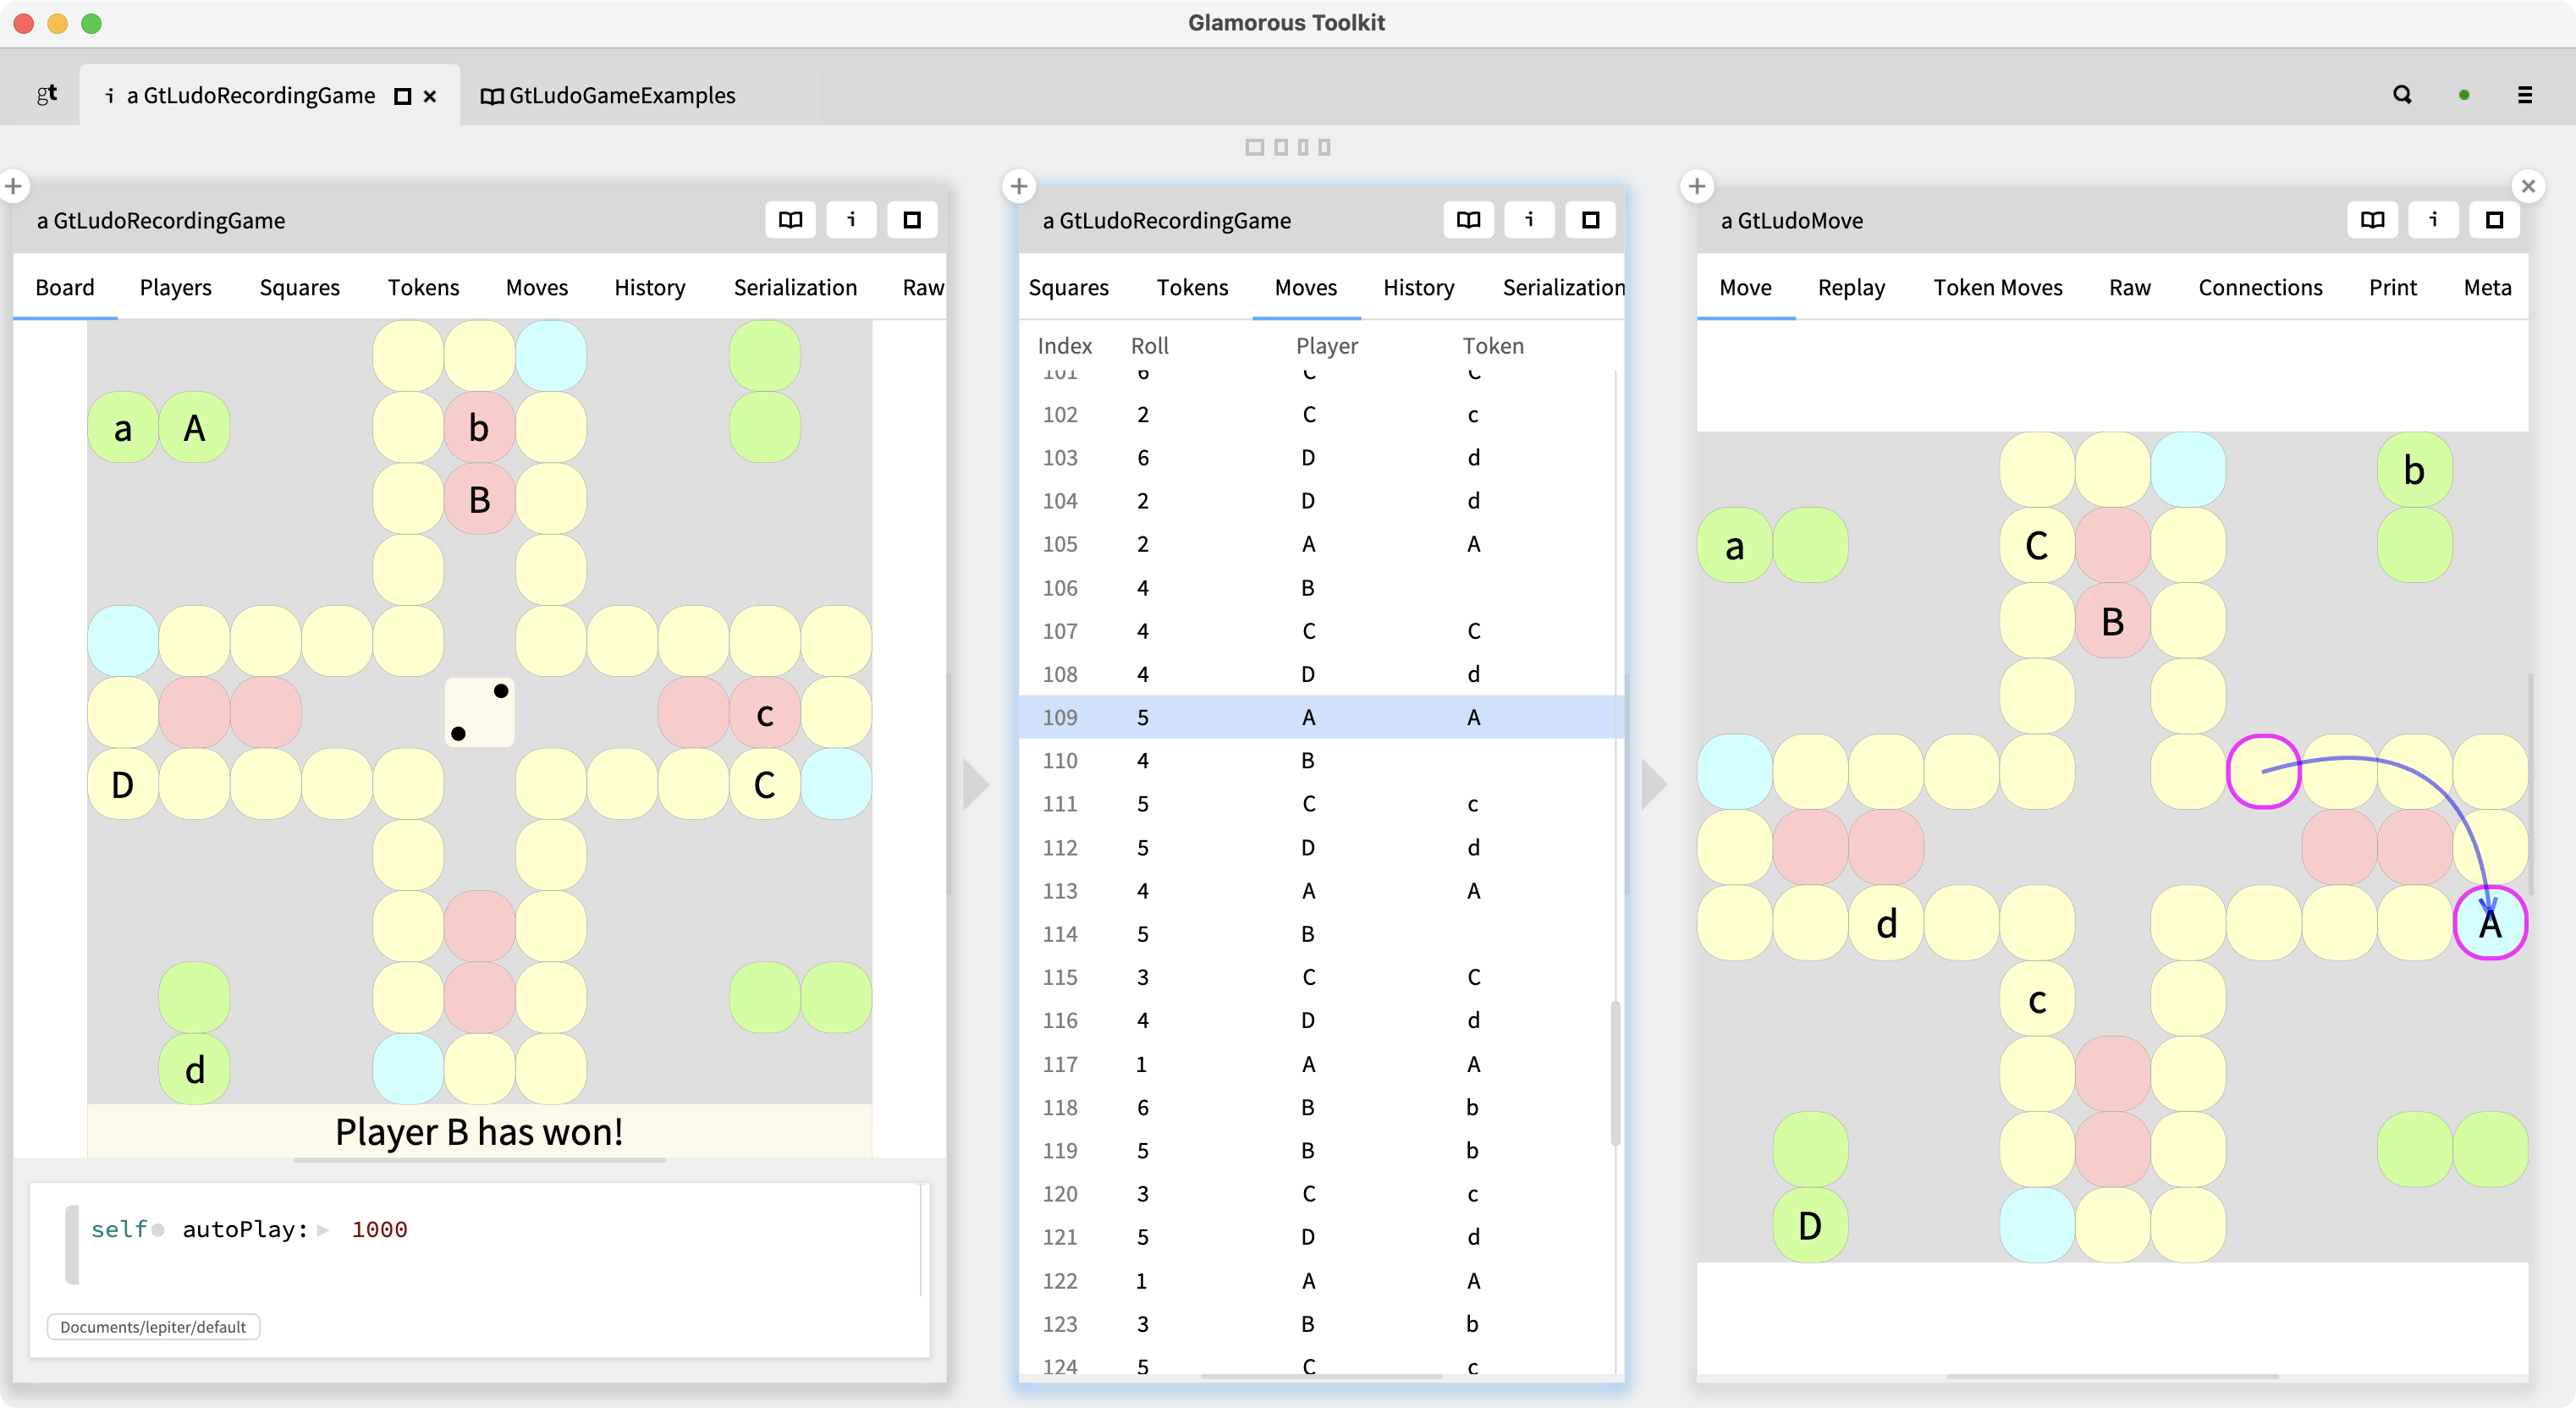
\includegraphics[width=\columnwidth]{customViews}
  \caption{Custom views of a Ludo game.}
  \label{fig:ludoViews}
\end{figure}

As a simple example, consider the inspector views of a Ludo game implementation in \autoref{fig:ludoViews}.
With a conventional implementation, we can either try to play the game interactively, or we can stare at the source code.
We can also run the tests, but if these are all green, they do not help us to understand the system.
By applying moldable development, we turn questions we have about the game into custom views.

The figure shows three connected custom inspector views of a running game in GT.
In the leftmost pane we see the game GUI as the \st{Board} view.
We can also interact programmatically with the game, evaluating ``\st{self autoPlay: 1000}'' in a contextual playground (a kind of interactive shell) below the view.
In the second pane we can explore the moves of  the completed game, and in the third pane we can explore individual moves.
The \st{Move} view visualizes the actual move performed in the context of the current game state at that point in time.
Each of these views is achieved with just a few lines of code, and leads to the Ludo game becoming an explainable system that can be explored in ways that are far richer and more intuitive than by trying to read source code.

In a nutshell, moldable development is a way to make systems explainable by making the \emph{inside} of a software system visible and explorable through custom tools.
Of course, this begs the question how to actually apply moldable development in practice.
In our experience applying moldable development to many industrial and open source systems, we have encountered a number of repeating patterns, which we document below.

% ===== Moldable Development Patterns =========================
\section{Moldable Development Patterns}

\rb{In our view, the paper is weakened by the assumption that it is aimed at the same audience as the previously published paper. Your goal in the "book" was to inform GT students of the scope of possibilities in this product. We would hope that your goal in publishing samples through PLoP would be to spread your success more broadly. (Ward is thinking of sharing with him for example). }

Moldable development can be understood in terms of a collection of mutually supporting 
patterns, in other words, a \emph{pattern language}, summarized in \autoref{fig:map}.
These patterns have emerged over several years of experience in developing \GT following moldable development, and applying it to numerous projects.

\begin{figure}[h]
  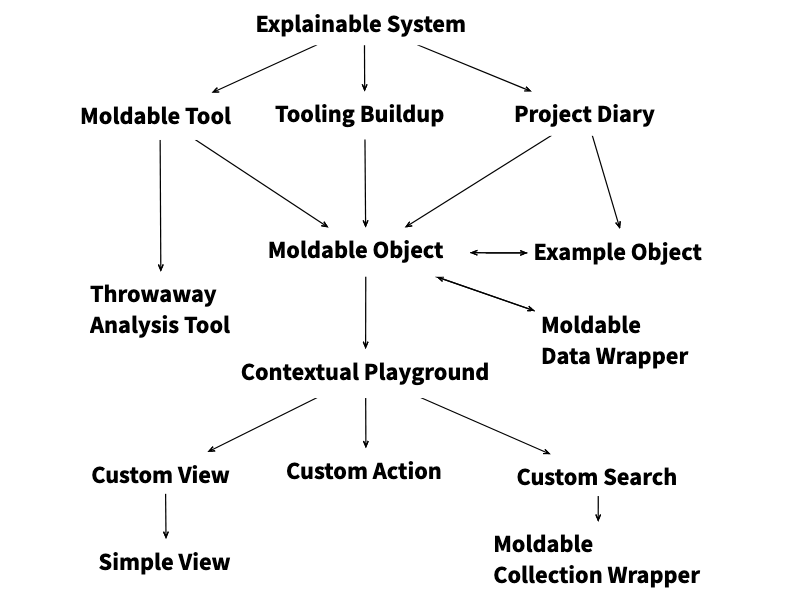
\includegraphics[width=\columnwidth]{map}
  \caption{A map of moldable development patterns.}
  \label{fig:map}
\end{figure}

\kh{What is not obvious from the description of the patterns is how they
mutually support each other. There's an opportunity for a follow-up
paper that describes how the patterns are applied in a real project.}

\eog{I think like that, the hard thing for this section number two that I found is that there's like a lot of definitions of what things are without a lot of connected motivation.
And it felt like I don't know if this is a thing that you've ever experienced, but you sit down you play, you're ready to play a board game with some friends and then someone's like, all right, we're gonna sit down and read the rule book from like cover to cover and then everything will be good.
And then you've got people like me who are like, what is the point of this game?
How do I win?
And then like from that I can gather, like my, I can interest my brain in the parts that matter.
And it's really tough to hold on to just like a list of definitions, for example, without that.}

The arrows in the diagram can be interpreted as meaning that one pattern ``uses'' or ``requires'' others.
The patterns that are concerned with \emph{Tooling} are tagged with ``(T)'', with \emph{Modeling} ``(M)'', and with the development \emph{Process} ``(P)''.

There are two distinct roles involved in moldable development:
\begin{inparaenum}[(i)]
\item the \emph{Facilitator} is responsible for the technical realization of custom tools, and
\item the \emph{Stakeholder} is responsible for the domain model and questions about the domain that should be answered by the custom tools.
\end{inparaenum}
In a purely technical domain, these two roles can often be played by the same person (\ie a developer), but in general they may be distinct people.

At the top of the map we have ``Explainable System,'' which is not a pattern per se, but rather the goal of moldable development.
An \empty{explainable system} is a software system whose domain model has been exposed with the help of numerous custom tools~\cite{Nier22a}.

Each custom tool can be seen as an extension of an existing \pattern{moldableTool}, which can be cheaply adapted by a simple customization.
Some domains require a preliminary phase of \pattern{toolingBuildup}, for example, to create dedicated parsers for programming languages, DSLs or specialized data formats, or bridges to other execution platforms.
A \pattern{blindSpot} is a problematic part of the target system that is hard to understand and work with, and may be a promising starting point for moldable development to initially engage Stakeholders.
A \pattern{projectDiary} is a notebook that serves as a starting point for development tasks.
A \pattern{throwawayAnalysisTool} can be a quick way to solve an urgent problem in a focused way.

Moldable development itself starts with a \pattern{moldableObject}, a live instance of a domain entity that is explored and molded with custom tools that package the results of exploration tasks.
An interesting instance can be encapsulated as an \pattern{exampleObject}, essentially a unit test that returns a tested object.
An example can be embedded in a project diary notebook page, and can also be used as a moldable object itself for further development tasks.
In case the domain includes already existing data entities, each of these can be wrapped in a \pattern{moldableDataWrapper} to produce a moldable object.

A moldable object can be explored with the help of its \pattern{contextualPlayground}, a live programming environment bound to the state of a live instance.
Working code can be extracted from such a playground to create custom tools.
The most common of these tools are:
\begin{inparaenum}[(i)]
\item a \pattern{customView}, a dedicated view of an object within a moldable tool such as an object inspector or a code browser, to display or visualize domain-specific information,
\item a \pattern{customAction} that encapsulates a useful domain action, and
\item a \pattern{customSearch}, to perform an ad hoc query over objects reachable from a given moldable object.
\end{inparaenum}
A custom view is frequently a \pattern{simpleView} that can be quickly prototyped, and later extended.
A custom search often benefits from a \pattern{collectionWrapper}, to allow the results of a query to be also molded with custom tools.

% ===== Tooling =========================
\section{Tooling Patterns}\label{sec:tooling}

We start by presenting the patterns that enable the cheap creation of custom tools.

\rb{Lots of folks like to compose patterns with a template. On wiki Ward suggested two paragraphs separated by the word "Therefore" was sufficient so long as the first paragraph described a recurring problem with roots in human nature, and the second paragraph described something specific you could make or do that "resolves" the forces present in the first paragraph. I might have referred to this as Patlets once or twice.}

\wc{Each statement describes how or where to apply a solution without explaining
what human need causes these solutions to be routinely required. We were led
to believe that an ability to make decisions is the root of each need. I will be
looking for ways to understand this decision making better and to tie human
decision making to the solutions offered by each pattern.}

% ----- Moldable Tool -------------------------
\subsection*{Moldable Tool}\label{pat:moldableTool}

\kh{My main criticism of the overall approach of presenting patterns is that
some of them aren't really patterns. For me, a pattern is something that
has been repeatedly observed in practice. The very first pattern you
present, "Moldable Tool", probably isn't a pattern. How many moldable
tools have been developed? I know of one.}

\subsubsection*{Context}
You are developing a software system, and find that the existing development tools fall short in supporting domain-specific questions about the software.

\subsubsection*{Problem}
How can you cheaply and effectively extend the development environment with domain-specific tools that address your application domain?

\subsubsection*{Forces}
Generic software tools are fine for answering generic questions, but they do not work well when addressing domain-specific questions.
For example, consider a generic debugger being used to debug an event-driven application\,---\,you want to step through the chain of events, not the stack.
A plugin architecture can open up an IDE to new tools, but plugins can be complex and expensive to implement, and they often do not play nicely with existing tools or with each other.

\tk{We call it "the preplanning problem" when discussing frameworks + plug-ins as an implementation option for software product lines. You need to identify all the hot spots for potential extensions in advance, define appropriate extension points, define interfaces which are not too broad and not too narrow, etc.}

\subsubsection*{Solution}
Make the development tools \emph{moldable} to the \emph{dynamic context} of the artifacts they are intended to work with~\cite{Chis17a}.

A moldable tool makes its core functionality configurable by means of lightweight mechanisms.
For example, a Test Runner in a modern IDE recognizes the presence of test cases by means of various programming conventions, \ie a test case is a method with a standard annotation, or it's a method whose name starts with ``\st{test}'' and belongs to a class that inherits from a \st{TestCase} class or implements a \st{Test} interface.

By the same token an inspector can be made moldable by recognizing that an object it is inspecting has one or more custom views defined as annotated methods.
For example, in \autoref{fig:viewCode} we see that inspecting an instance of a \st{GtLudoRecordingGame} yields a custom \st{Moves} view listing the moves played thus far, as the inspector detects a \st{gtMovesFor:} method defined in the object with a \st{<gtView>} pragma (\ie annotation).\footnote{All the examples are written in Pharo Smalltalk, the platform upon which \GT is built. See \url{https://pharo.org}}
The custom view is defined in a just a few lines of code, creating a \st{columnedList} from the moves.

\begin{figure}[h]
  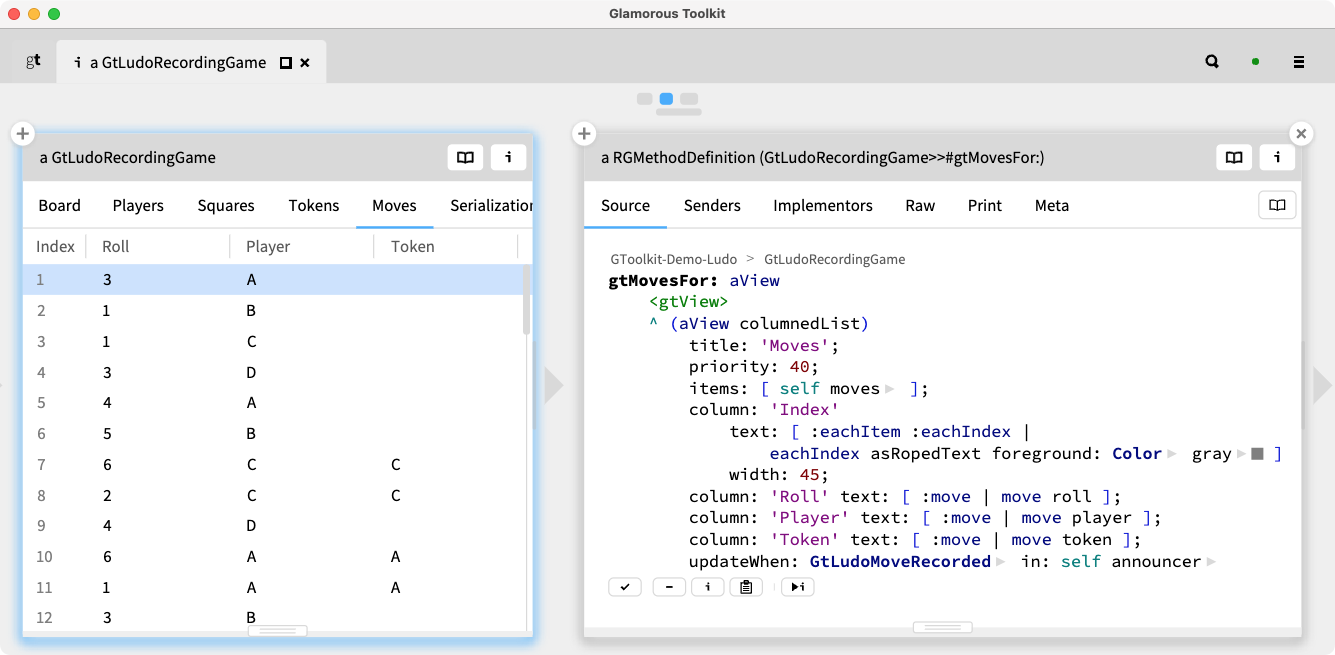
\includegraphics[width=\columnwidth]{viewCode}
  \caption{Defining a custom inspector view.}
  \label{fig:viewCode}
\end{figure}

The precise mechanism used to mold a tool is not as important as is the fact that the customizations should be cheap, \ie few lines of code, and \emph{dynamic}, \ie detected at run time.

Other examples include:
\begin{inparaenum}[(i)]
\item a moldable code browser offering alternative views of packages, classes or methods to show dependencies, tests, or other more domain-specific features,
\item a moldable debugger to adapt the stepping behavior for domains such as event-driven applications, or parsing rules, or
\item a moldable notebook, supporting domain-specific snippets or annotations.
\end{inparaenum}

\subsubsection*{Consequences}
A moldable tool requires no up-front configuration, since it will be dynamically molded by the artifacts it encounters.
Conversely, since custom tools are an intrinsic part of software systems rather than the IDE, molding happens when needed.
Some tooling effort is required to open up the existing IDE tools to make them moldable, \ie dynamically customizable.

% ----- Contextual Playground -------------------------
\subsection*{Contextual Playground}\label{pat:contextualPlayground}
\kh{"Contextual Playground" is a pattern, but I'd label it "process" rather
than "tooling". On the other hand, it's also reasonable to have it right
before "Custom View", as it's a preparation to tooling work.}
\subsubsection*{Context}
You have a moldable object, and you are ready to start exploring.

\eog{So you're exploring maybe we could talk about what, what exploring means.
Like if you ask a regular developer, like tell me about the explorations you've done this morning, versus, hey, what kind of like debugging or like learning about the system?}

\subsubsection*{Problem}
Where do you start coding?

\subsubsection*{Forces}
An editor for coding new methods typically provides no facilities for testing the code.
When we code new behavior as methods, we must repeatedly change our context to incrementally develop the logic.
Testing the code requires a separate setup.
Setting up code to prototype and test logic can be cumbersome.
Writing tests first for parts of the logic of a complex method can be overkill.

\subsubsection*{Solution}
Prototype new behavior in the contextual playground of the inspector on a \pattern{moldableObject}.
The playground will be bound to the context of the instance, so \st{self} and all slots (\ie instance variables) can be accessed exactly as they would in a running method.
From the moldable object you can navigate to any parts of the instance, to explore the APIs, or to test experimental code.
Code snippets that work as expected can then be copy-pasted to existing methods, or extracted to new methods using an \emph{Extract method} refactoring~\cite{Fowl99a}.

In \autoref{fig:inspectingPythonObjects} we see an inspector view of an instance of a Python \st{MovieCollection} class.

\begin{figure}[h]
  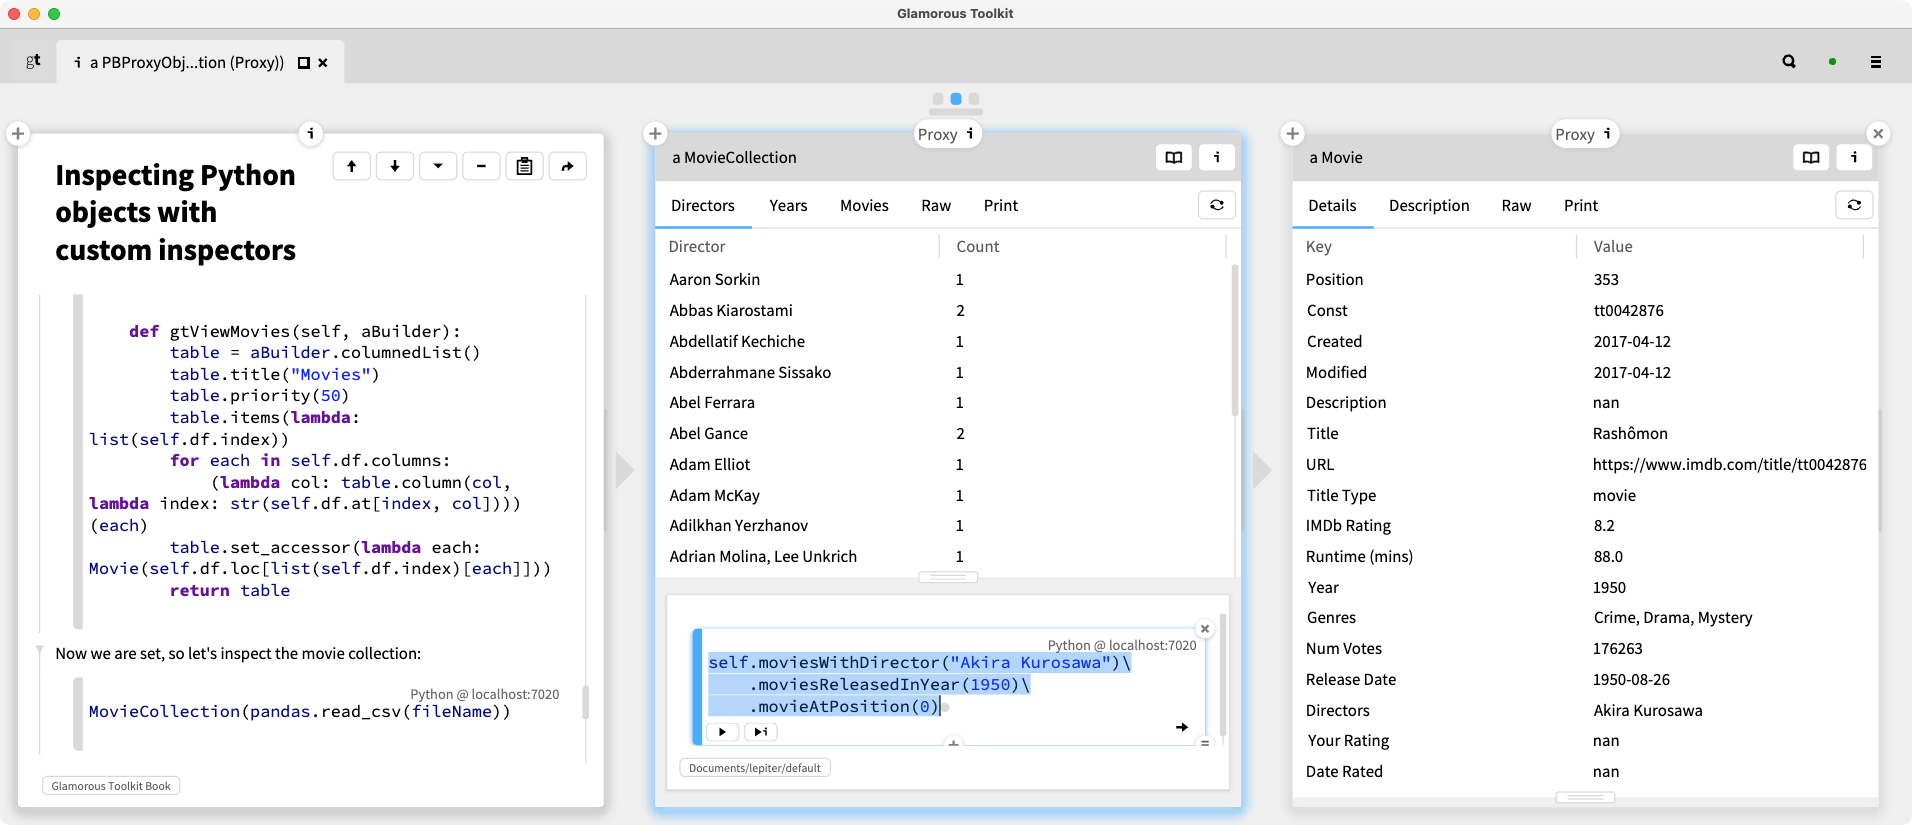
\includegraphics[width=\columnwidth]{inspectingPythonObjects}
  \caption{Exploring Python objects in a contextual playground.}
  \label{fig:inspectingPythonObjects}
\end{figure}

In the contextual playground we experiment with Python code to extract a particular movie.
We use a \pattern{customView} of the \st{MovieCollection} and of the \st{Movie} to aid our exploration.
Note that \st{self} in the code snippet is bound to the context of the \st{MovieCollection} instance.
Once we have identified some useful code, we can extract it as a new method of the object.
Similarly, if we identify an interesting instance, we can use the code to define an \pattern{exampleObject}.

A well-known use of contextual playgrounds is the JavaScript console of a modern web browser: while inspecting a live web page, you can explore and programmatically interact with the live objects in the run-time environment of the page.

\subsubsection*{Consequences}
By prototyping new behavior in a contextual playground, you obtain immediate feedback for experimental code.

% ----- Custom View -------------------------
\subsection*{Custom View}\label{pat:customView}
\subsubsection*{Context}
You are exploring a live domain model and find some interesting information.

\subsubsection*{Problem}
How do you make it easy to find interesting information again?

\subsubsection*{Forces}
Navigating to the data you want to reach may entail a sequence of operations, either clicking in views, or evaluating Playground snippets, to reach the answer you seek.
The sequence of steps may be cumbersome to follow repeatedly.

\eog{this part here, you could describe it also with like a watch statement in javascript or whatever, like this kind of thing.
And then people could be more familiar with that because they, they do that.}

\subsubsection*{Solution}
Turn interesting data into a custom view.
Extract the navigation steps into a new custom view for the moldable object you start navigating from.
Start with a \pattern{simpleView}.

\eog{I'd love to see maybe a picture like a figure with this.}

As an example, consider the views of a partially played Ludo game in \autoref{fig:rawViewVsCustomView}.
We would like to understand which moves have been played up to now.
In the leftmost pane we are exploring a ``raw view''\,---\,a generic view of the state of the object.
With this view we can navigate to the individual moves and explore them, but it is a clumsy way to explore the object.
In the second pane we see a custom \st{Moves} view that lists the moves in order, with columns showing each roll of the die, the player who rolled the die, and any token that may have moved.
From this custom view we can furthermore dive directly into the \st{Move} object, which in turn has a custom view visualizing the change in state.

\begin{figure}[h]
  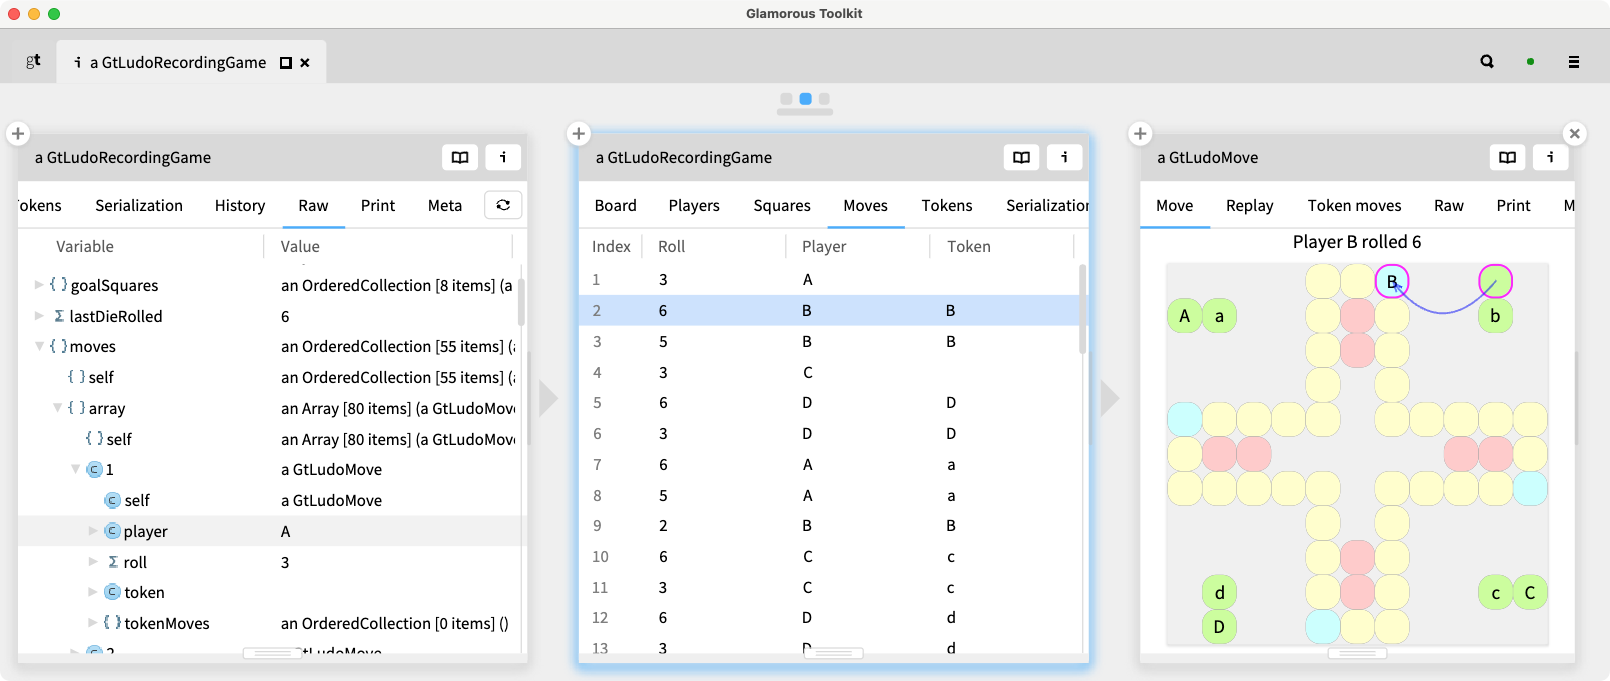
\includegraphics[width=\columnwidth]{rawViewVsCustomView}
  \caption{A raw view and two custom views.}
  \label{fig:rawViewVsCustomView}
\end{figure}

\subsubsection*{Consequences}
A custom view exposes information about a domain that can otherwise be hard to find.
Custom views become an intrinsic part of a software system, thus turning it into an \emph{explainable system}.
You need a \pattern{moldableTool} into which you can dynamically plug custom views.

\eog{Down here, there's mention of what a you need a moldable tool, but I still don't understand what a moldable tool is given just this paper so far.}

% ----- Custom Search -------------------------
\subsection*{Custom Search}\label{pat:customSearch}
\subsubsection*{Context}
You have a complex domain model consisting of various kinds of entities related to each other.

\subsubsection*{Problem}
How can you effectively navigate between domain entities by name, content or other criteria?

\subsubsection*{Forces}
It can be hard to anticipate which domain  entities you will need to navigate to.
Designing a good query interface can be a difficult task.

\subsubsection*{Solution}
Add a custom search for every kind of domain entity you want to navigate to.
Simply search by substring against various attributes of the domain objects.
Add a separate search for each attribute type or domain object.

In \autoref{fig:customSearch} we see several custom searches for page names, page content and link names within a website.

\begin{figure}[h]
  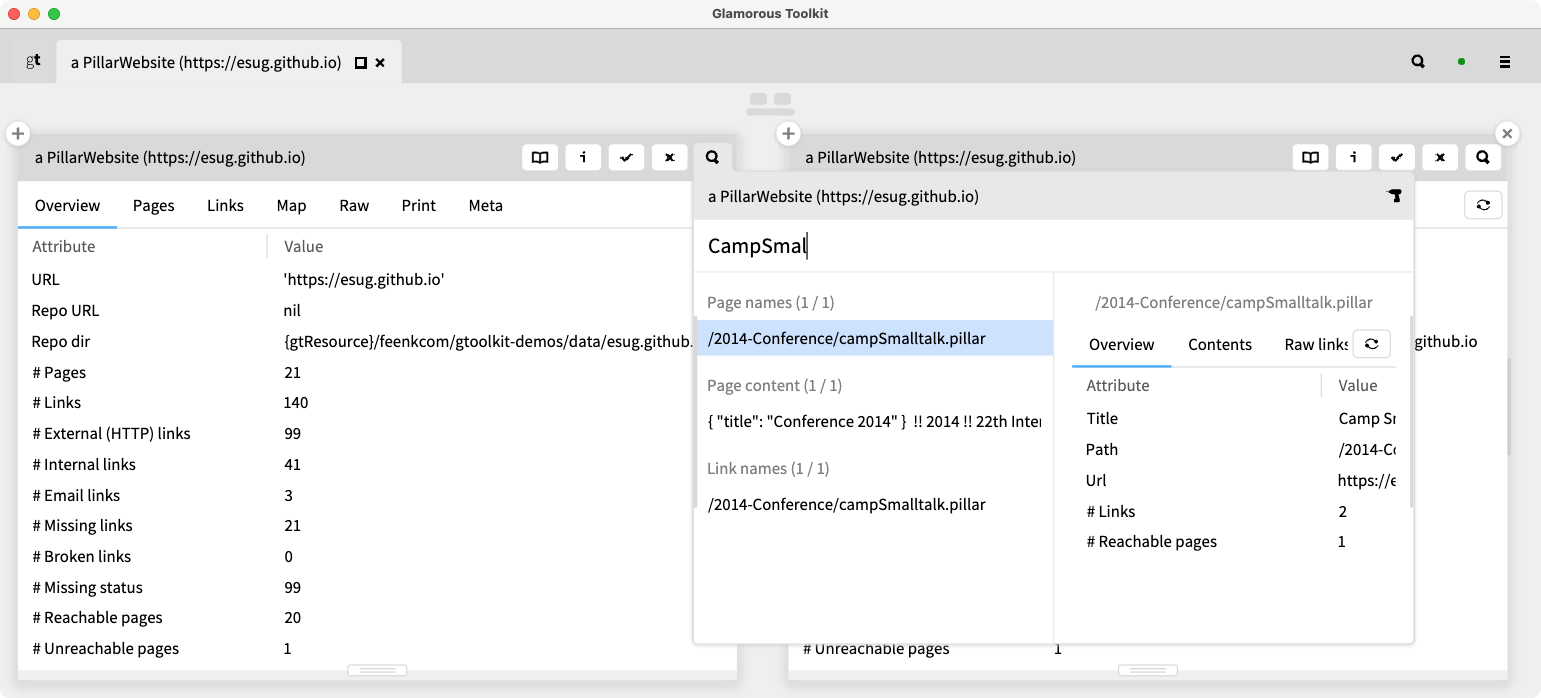
\includegraphics[width=\columnwidth]{customSearch}
  \caption{Custom substring searches.}
  \label{fig:customSearch}
\end{figure}

\eog{I think what I was curious about is if there is a way to use an example of a domain specific custom search example, that would be really cool.
So I don't know, maybe something in ludo or like something more than just like researching.}

As with other custom tools, one way to implement a custom search is as a method of the domain object from which the search is initiated, with a dedicated annotation.
In \GT, custom searches are annotated with \st{<gtSearch>}, and triggered within multiple moldable tools, such as the inspector, the code editor, and also the notebook.

\subsubsection*{Consequences}
You need a \pattern{moldableTool} into which you can dynamically plug custom searches.
The same search interface can accommodate multiple custom searches to query different attributes of multiple domain entities.

% ----- Custom Action -------------------------
\subsection*{Custom Action}\label{pat:customAction}
\subsubsection*{Context}
You are developing an explorable domain model of your application and find yourself repeatedly evaluating the same code snippets to perform a certain action or navigate to another object.

\subsubsection*{Problem}
How can you streamline execution of repeated actions?

\subsubsection*{Forces}
Repeated tasks are annoying and time-consuming.
Remembering how to perform common tasks increases cognitive overload.
Storing code to perform common actions as methods or as snippets in class comments doesn't guarantee that the code will be easily found when you need it.

\subsubsection*{Solution}
Add a custom action button to the moldable tool for the object involved in a repeated task, encapsulating the boilerplate code to perform it.
Be sure to pick an evocative button icon and tooltip text to make the intent of the button clear.
Only add buttons for the most important actions to avoid cluttering the interface of a moldable tool.

As an example, consider the inspector view in \autoref{fig:customLePageAction} of a notebook page in Lepiter~\cite{Girb21a}, the live documentation system of GT.
Common actions are to navigate to the notebook database, to view the file in which the state of the notebook page is stored, or to export an HTML version of the page.
Each of these actions can easily be packaged as an inspector button, so that the action can be performed with a single click, opening a new inspector view of the result.
In the example we navigate to the database holding all related notebook pages for the given project.

\begin{figure}[h]
  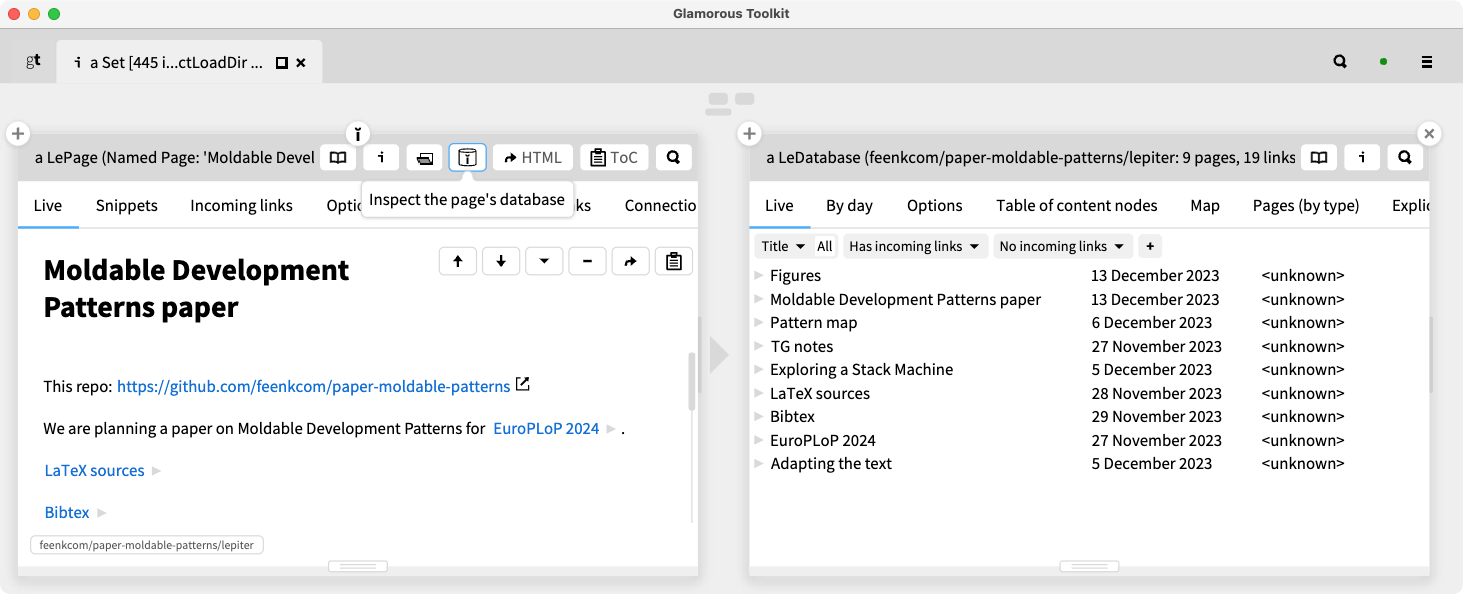
\includegraphics[width=\columnwidth]{customLePageAction}
  \caption{Custom actions for Lepiter pages.}
  \label{fig:customLePageAction}
\end{figure}

\subsubsection*{Consequences}
Custom actions appear as buttons in moldable tools only in the context of the objects to which they can be applied.
You need a \pattern{moldableTool} into which you can dynamically plug custom actions.

% ===== Modeling =========================
\section{Modeling Patterns}\label{sec:modeling}

Next we present the patterns related specifically to modeling domain entities in a way that facilitates querying and exploration of an explainable system.

% ----- Moldable Object -------------------------
\subsection*{Moldable Object}\label{pat:moldableObject}

\subsubsection*{Context}
You are ready to start the process of creating an explainable system, either from scratch, or based on some existing software or data.

\subsubsection*{Problem}
Where do you start coding an explainable system?

\subsubsection*{Forces}
As a programmer, you want to quickly get feedback about the code you are writing.
When you write code in a conventional code editor, you are several steps away from seeing the consequences of your coding.
To write unit tests, you must already know what behavior you want to test and what the results should be.

\subsubsection*{Solution}
Start coding by inspecting a moldable object, that is, a live instance of the class you are coding, \emph{not in a code editor}.
Then incrementally pose domain-specific questions, find the answers by exploring and interacting with the object, and then turn those answers into custom tools, behaviors and tests.

Moldable development is about making systems explainable with the help of custom tools, which means that you need to start the process by asking questions that you want to answer.
In most cases you can't immediately start building the custom tools, but rather you need to explore the domain objects to understand how to answer the question.
Once you know how to get the answer, you can turn the exploration steps into a custom tool.
Starting with a live object means that you can immediately start the exploration process.
Turning the exploration of an object into a custom tool is the process of molding it, hence we call it a ``moldable object.''

How do you obtain a moldable object?
\begin{itemize}[---]
\item \emph{You already have a class:} create a \pattern{projectDiary} notebook page containing a code snippet to create an instance of the class, and start from there.
\item \emph{You don't have a class:} start instead with a code snippet that instantiates an empty class, and then prototype the behavior.
\item \emph{You have a test case:} turn the test case into an \pattern{exampleObject} and start from there.
\item \emph{You have some data:} wrap the data as a \pattern{moldableDataWrapper}.
\end{itemize}

In \autoref{fig:moldableLudoGame} we see an Inspector on an instance of a \lst{Gt\-Ludo\-Recording\-Game} with a \pattern{contextualPlayground} where we can write experimental code that we later extract as methods.
In this case we are prototyping the \emph{autoplay} feature.
In the second pane we see the \emph{History} view of the object, showing the details of all the moves of the game.

\begin{figure}[h]
  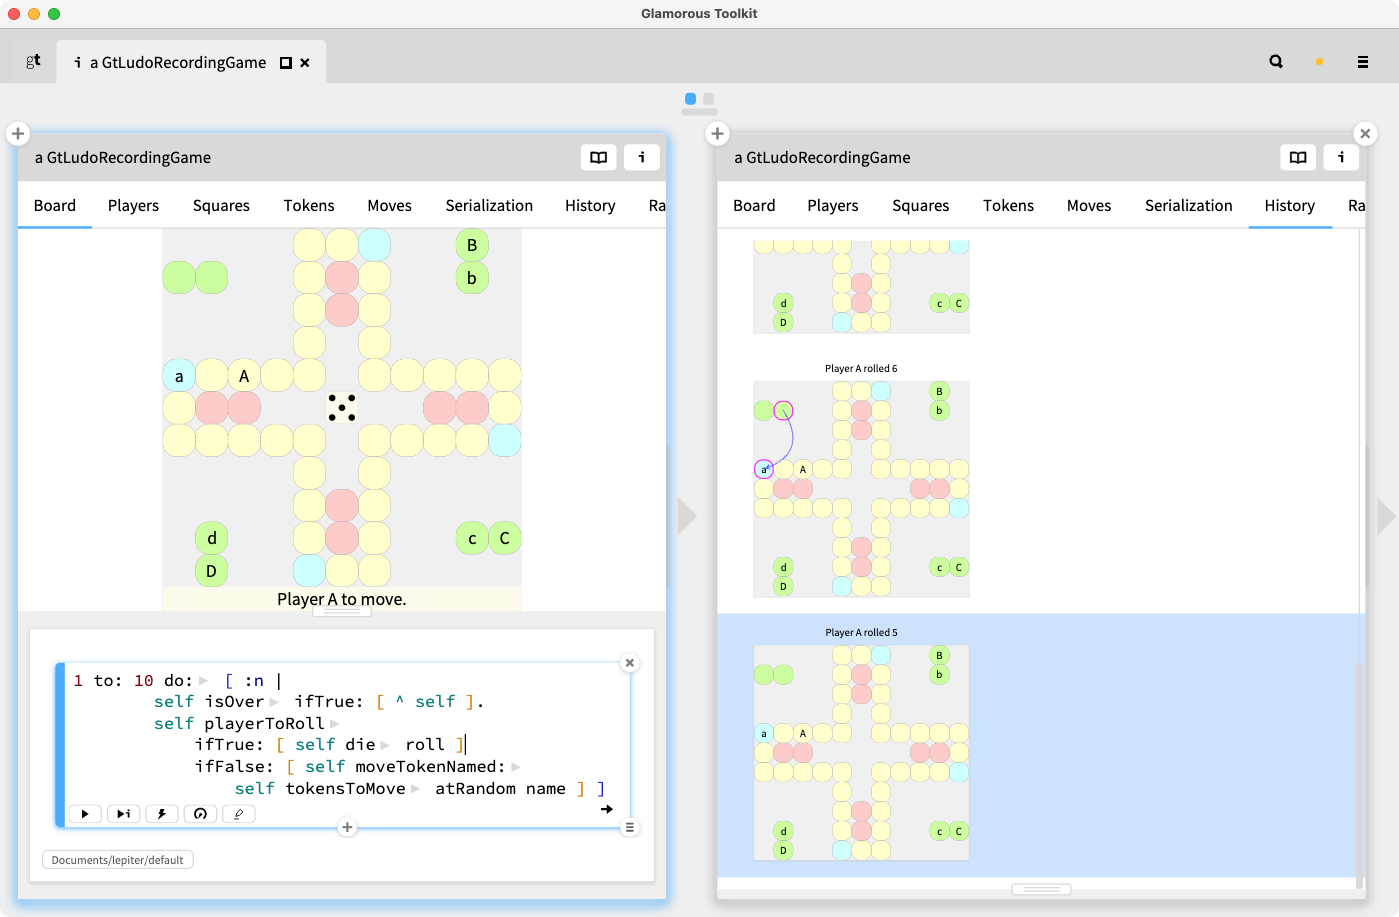
\includegraphics[width=\columnwidth]{moldableLudoGame}
  \caption{A moldable Ludo game instance.}
  \label{fig:moldableLudoGame}
\end{figure}

With the moldable object at hand, we can ask questions like \emph{What is the current state of the Ludo game?}, or \emph{What happened in the last few moves that we autoplayed?}
As we answer questions we can create small custom tools, such as a \pattern{customView} or a \pattern{customAction}.
Whenever we identify an interesting state of our moldable object, we can extract it as an \pattern{exampleObject} that we can use as a test case, or as a starting point for further moldable development.

\subsubsection*{Consequences}
Instead of writing code in a text editor in the context of the source code of a class, you are always working in the context of a live object, whose behavior can be immediately explored.
Instead of writing hypothetical code that you must afterward test, you start by prototyping code, and then extracting new behavior.
Instead of trying to program custom tools in a vacuum, you first explore and prototype answers to questions, and then extract the code you need to create a custom tool.

% ----- Example Object -------------------------
\subsection*{Example Object}\label{pat:exampleObject}
\subsubsection*{Context}
You want to explore questions about domain objects that are in particular execution states.

\subsubsection*{Problem}
How do you create an object in a particular state to start a moldable development task?

\subsubsection*{Forces}
Concrete examples are needed for many purposes, such as documentation, testing, and exploration.
Examples can be complex to set up.
Unit tests consume examples, but they are only accessible if a test fails.

\subsubsection*{Solution}
Wrap examples as (instance) methods that optionally evaluate some tests (assertions), and return the example instance.
Each example may also use one or more existing examples as the initial setup to arrive at the new execution state.

To start, you need a modified unit testing framework in which tests return the exercised fixture, namely, an example.
In GT, you create an example by defining a parameterless method that has a \st{<gtExample>} pragma and returns an object.
A similar framework for Java is JExample~\cite{Kuhn08a}.

Here is a simple example method that creates a fresh instance of the \st{gtLudoGame} class, asserts a few basic facts (\ie that the game is not yet over, no one has won yet, and so on).
It resembles a classical unit test in all respects except one: it returns the instance of the unit under test, \ie the \st{game} instance.

\needlines{5}
\begin{code}
GtLudoGameExamples>>#emptyGame
	<gtExample>
	| game |
	game := self gameClass new.
	self assert: game isOver not.
	self assert: game winner equals: 'No one'.
	self assert: game currentPlayer name equals: 'A'.
	self assert: game playerToRoll.
	self assert: game playerToMove not.
	^ game  "return the game instance"
\end{code}

Unlike normal test methods, examples are designed to be \emph{composed}.
In \autoref{fig:composedExample} we see a second example, \st{playerArolls6}, that starts from the \st{emptyGame} example, rolls a $6$, asserts a few facts, and returns the modified game instance.

\begin{figure}[h]
  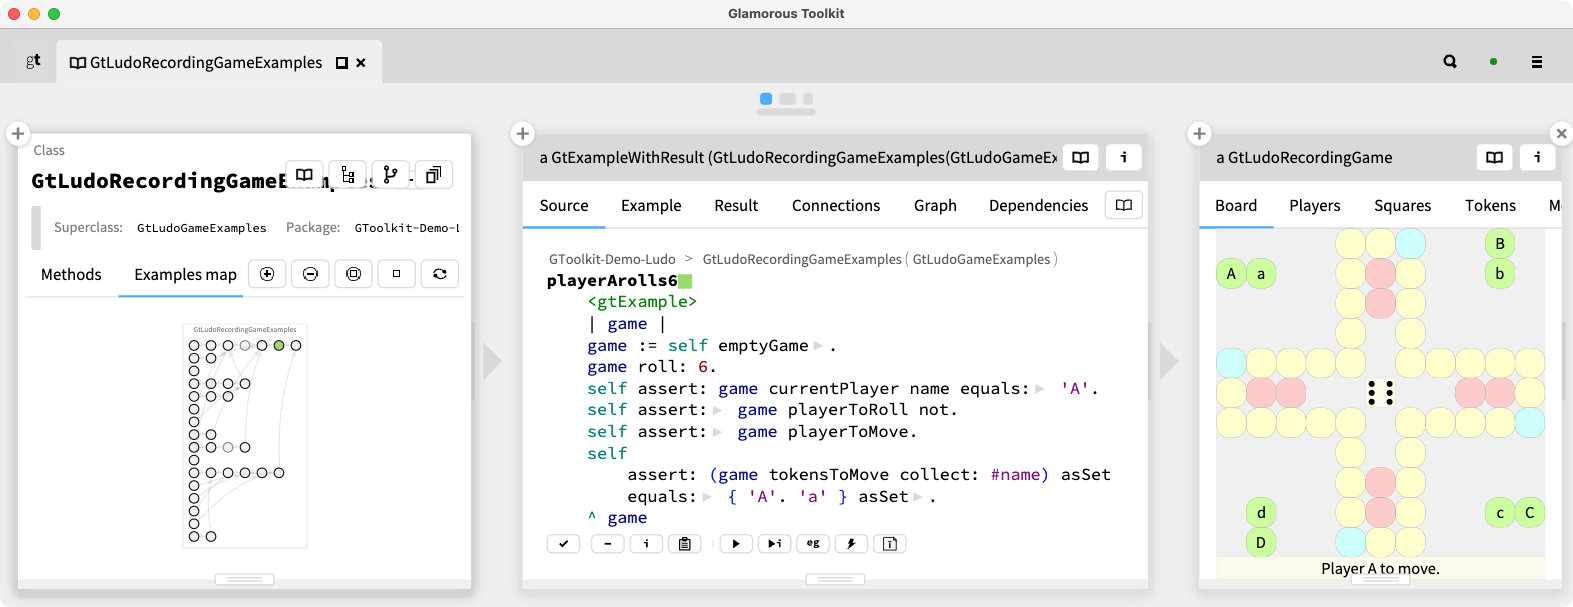
\includegraphics[width=\columnwidth]{composedExample}
  \caption{Composing examples.}
  \label{fig:composedExample}
\end{figure}

Examples such as these can be embedded into notebook pages and used as moldable objects for further development tasks, or as documentation, as seen in \autoref{fig:documentingLudo}.

\begin{figure}[h]
  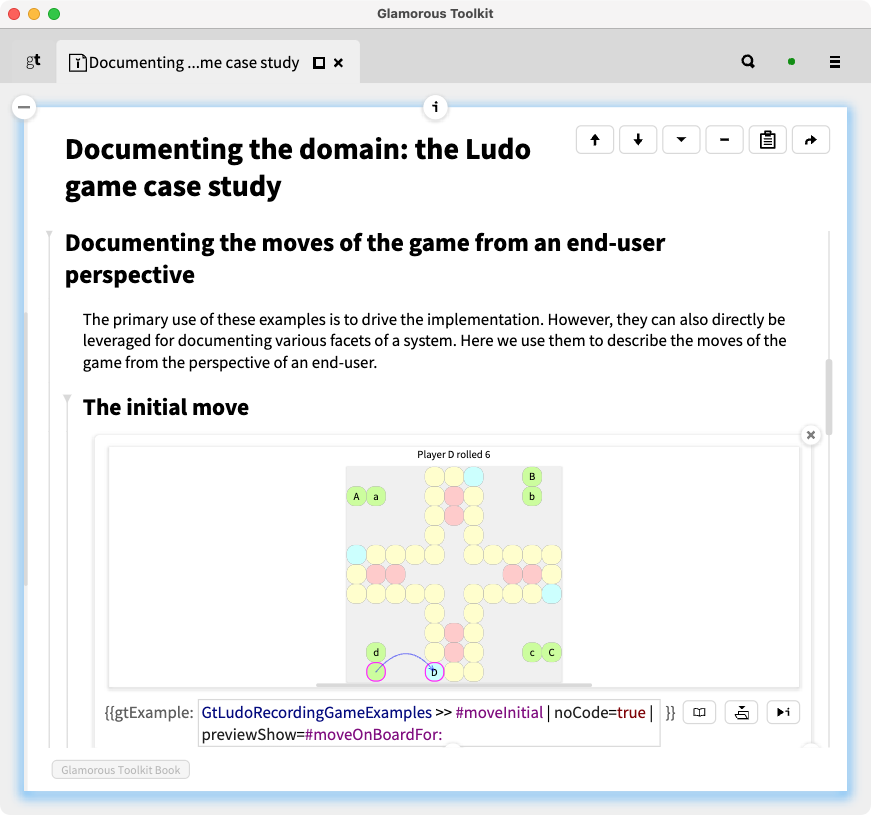
\includegraphics[width=\columnwidth]{documentingLudo}
  \caption{Documenting the Ludo game with live example objects.}
  \label{fig:documentingLudo}
\end{figure}

    
\subsubsection*{Consequences}
Examples can be run just like classical unit tests.
When an example fails, its dependent examples do not need to be run.
When an example succeeds, it can be inspected, used as a moldable object to start coding, or embedded as a live example snippet within a notebook page to illustrate some point.
When you are searching for usages of an API, not only do you find examples that illustrate the usage, but by running the example you obtain a live instance that you can explore.

% ----- Moldable Data Wrapper -------------------------
\subsection*{Moldable Data Wrapper}\label{pat:moldableDataWrapper}

\subsubsection*{Context}
You are working in a domain with existing data that you want to turn into an explainable system.

\subsubsection*{Problem}
How do you develop custom tools for existing data?

\subsubsection*{Forces}
When we explore data, we represent them using suitable low-level data structures.
Data structures (lists, dictionaries) reflect the representation of data, not their interpretation.
To analyze and explore data, we need higher-level views that reflect our understanding of the data.

\subsubsection*{Solution}
Wrap each kind of data using a dedicated class reflecting the problem domain entity.
As you explore the data, introduce custom tools (views \etc) to the domain class that reflect answers to questions you ask about the data.

First extract the data of interest.
This might be data sitting in your file system (for example, a CSV file), or data retrieved from a website.
For example, here we retrieve a \st{Dictionary} representation of JSON data about the feenk GitHub organization:

\begin{code}
url := 'https://api.github.com/orgs/feenkcom'.
json := ZnClient new get: url.
dictionary := STON fromString: json.
\end{code}

\eog{Would love to see the goal or motivation earlier for this kind of jazz.}

The dictionary representation, however, is not well-suited for exploring the GitHub organization domain.
If we explore the resulting object (see \autoref{fig:rawGitHubData}) we just see the keys and values of the raw downloaded data.
From this view, of course we can explore the data by navigating the Dictionary views, or by programatically exploring other paths, but we cannot add or tailor views to specifically support the GitHub Organization domain.

\begin{figure}[h]
  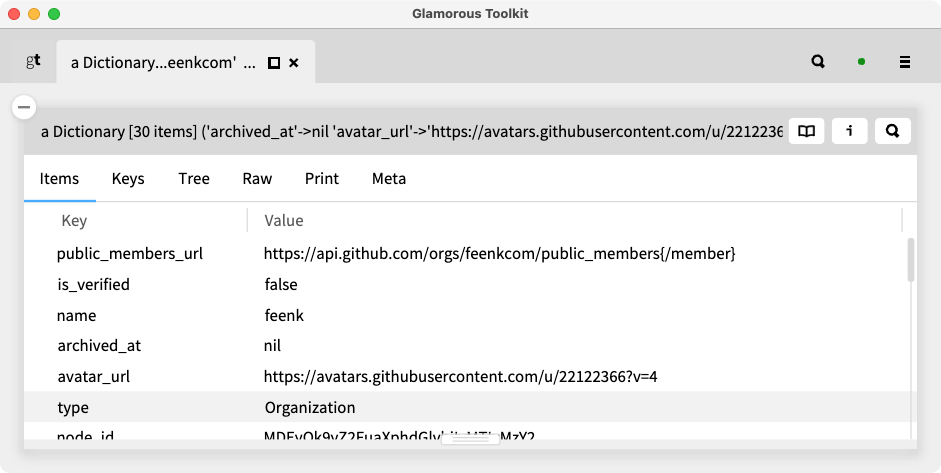
\includegraphics[width=\columnwidth]{rawGitHubData}
  \caption{Raw (not moldable) GitHub data.}
  \label{fig:rawGitHubData}
\end{figure}

We address these problems by wrapping the raw data as a dedicated \st{GhOrganization} object, as follows:

\begin{code}
GhOrganization new rawData: dictionary.
\end{code}

Now we can add custom views specific to this domain, for example, listing the repositories of an organization, or the most recent GitHub events.
For each new domain concept, we introduce a dedicated wrapper object, so we can navigate the entire model via the domain concepts.
We see the result after some moldable development steps in \autoref{fig:wrappedGitHubData}.

\begin{figure}[h]
  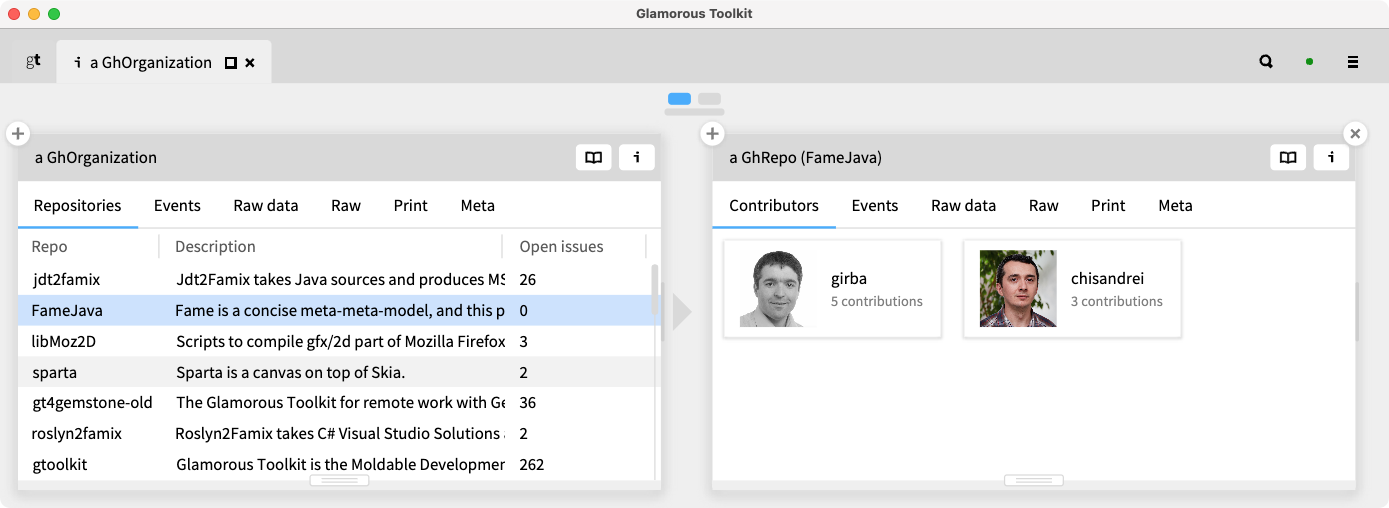
\includegraphics[width=\columnwidth]{wrappedGitHubData}
  \caption{Wrapped (moldable) GitHub data.}
  \label{fig:wrappedGitHubData}
\end{figure}

\subsubsection*{Consequences}

By wrapping the raw domain data, you obtain a moldable object that can be customized to form part of an explainable system.
Each time you navigate to other data representing further domain entities, wrap them as well, to build an explorable domain model.
In case custom tools of the underlying data objects are useful, you can always recycle them and make them available to the wrapped objects as well.

% ----- Moldable Collection Wrapper -------------------------
\subsection*{Moldable Collection Wrapper}\label{pat:collectionWrapper}

\subsubsection*{Context}
Within your application domain, you not only have to deal with individual domain objects, but also composite entities (\eg a book of notebook pages, a website of web pages), and collections of entities (\eg the result of query).

\subsubsection*{Problem}
How can you effectively provide custom tools for various kinds of collections of domain entities?

\subsubsection*{Forces}
Collections are generic data structures with generic views that are not necessarily informative for your domain.
Collections of domain entities may occur in various forms and contexts, such as the state of a composite object, or the result of a query.
Providing custom views for each of these can be tedious and lead to much duplicated code.

\subsubsection*{Solution}
Wrap a collection of domain objects in a dedicated collection wrapper, and give it dedicated views, actions and searches.
In case there are multiple composite entities or collections that should share the same custom tools, factor these out into a common abstract superclass or trait~\cite{Duca06b}.

For example, in \autoref{fig:moldableCollectionWrapper} we see that when we navigate to the \st{Pages} of a website, we obtain not a raw collection, but a \lst{Web\-Page\-Group} wrapping the collection, and providing custom tools, such as a map of reachable and unreachable pages.
Similarly, a query for pages matching a particular string will also return a wrapped group with dedicated tools.

\begin{figure}[h]
  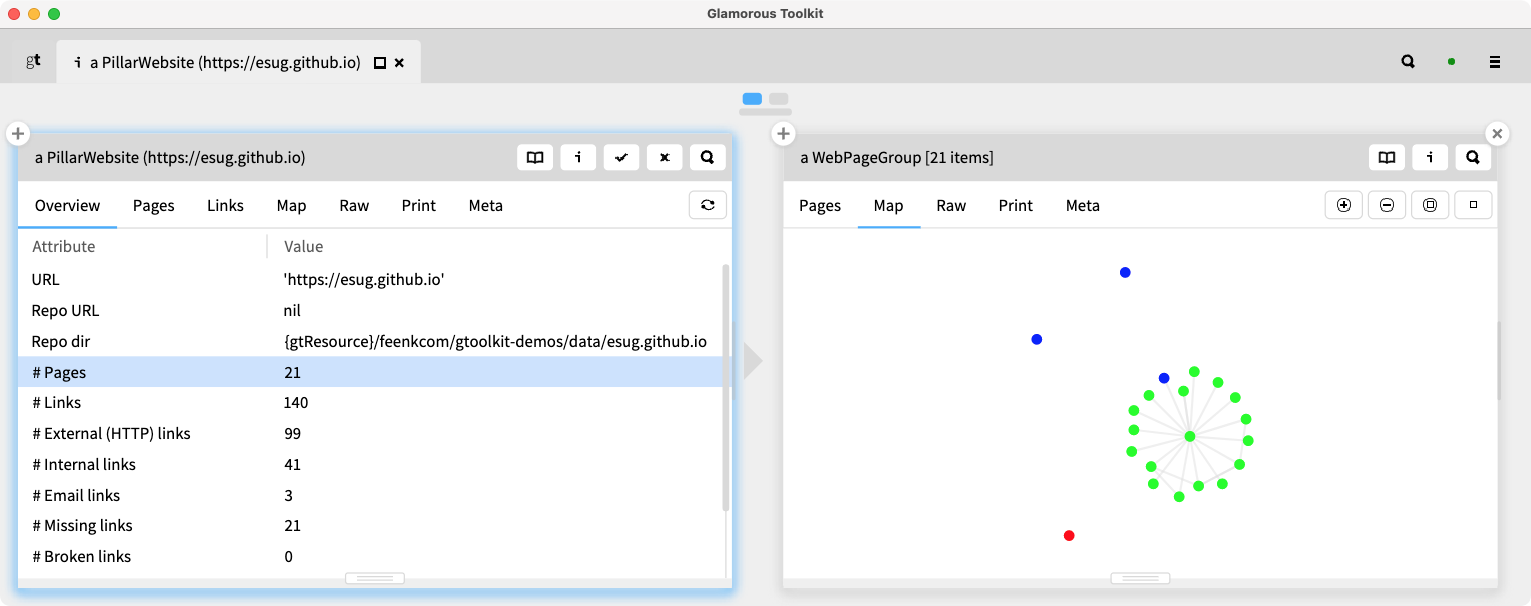
\includegraphics[width=\columnwidth]{moldableCollectionWrapper}
  \caption{A moldable collection wrapper for web pages.}
  \label{fig:moldableCollectionWrapper}
\end{figure}

Furthermore, if the wrapped collection or composite object should also behave like a collection, use a trait to forward collection API requests to the underlying collection.
In this example, \st{WebPageGroup} uses the trait \st{TGtGroupWithItems} that forwards all collection requests to the \st{items} slot of the wrapper that holds the raw collection.

\subsubsection*{Consequences}
Composite domain objects and collections of domain objects can be molded to support custom tools.
Query results can be similarly molded.
Wrapped collections can be made plug-compatible with raw collections.

% ===== Process =========================
\section{Process Patterns}\label{sec:process}

We conclude with the process patterns that provide guidance in organizing and steering moldable development tasks.

% ----- Project Diary -------------------------
\subsection*{Project Diary}\label{pat:projectDiary}

\subsubsection*{Context}
You are working on a software project and need to track your progress.

\subsubsection*{Problem}
How can you keep track of decisions, experiments and progress in a moldable development project?

\subsubsection*{Forces}
It's boring to write documentation after the fact, so it is rarely done.
Documentation is not part of the running system, so it distracts you from coding.
Tools for tracking your progress are separate from the code base, so they are commonly out of sync with reality.

\subsubsection*{Solution}
Use a live notebook as the starting point for all tasks.
Create a dedicated notebook page for each project, or even each project task, to summarize the goals, and provide pointers to related material.
Use the notebook to keep a diary of your progress.

As the project matures, use the notebook as a draft for the documentation.
For example, in \autoref{fig:projectDiary} we see a live Lepiter page in the \GT Book\footnote{The GT Book is the documentation of the Glamorous Toolkit Moldable Development Environment implemented as a live Lepiter notebook. An archived static snapshot of this page is also available: \url{https://web.archive.org/web/20231213144857/https://book.gtoolkit.com/adding-simple-list-views-for-ludo-players--3g9kpmxty3fj9eev3ucmqkztc}.} documenting the task of adding some list views to the Ludo game.

\eog{``Using a live notebook.'' I know folks maybe in like Jupiter like Python stuff but specific kind of like scientific Python are used to using this word or this phrase, but I would explain it or define it if you can, if you if you have the space.}

\begin{figure}[h]
  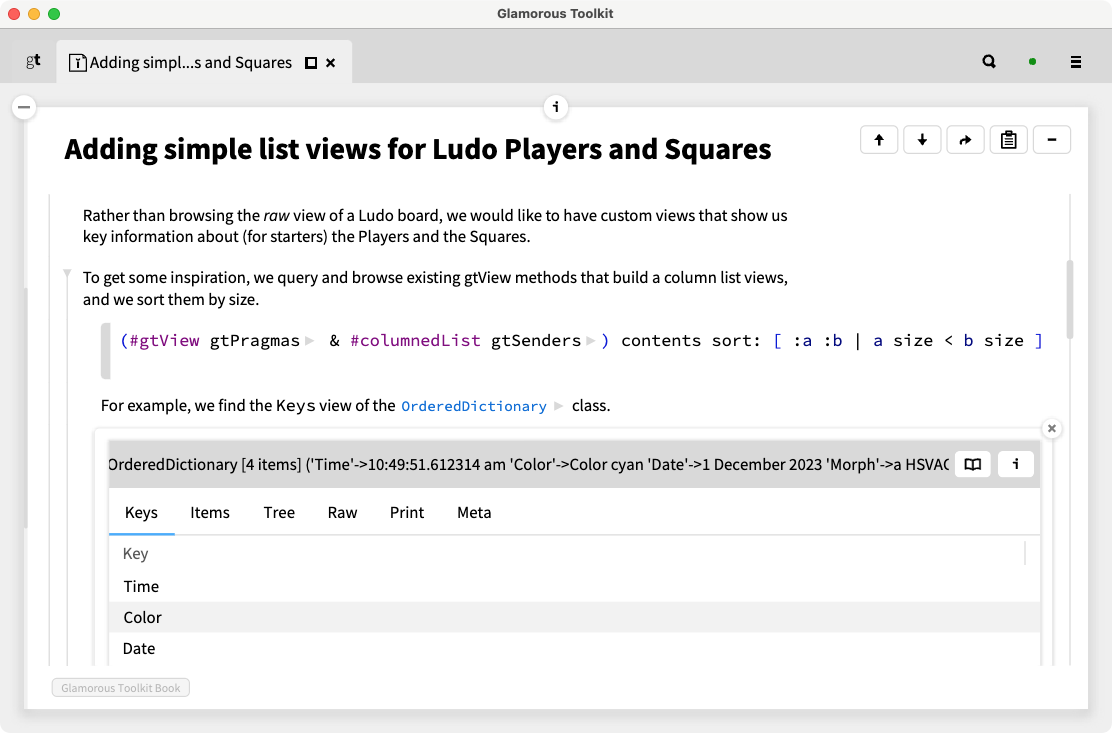
\includegraphics[width=\columnwidth]{projectDiaryExample}
  \caption{Documenting your progress in a live notebook.}
  \label{fig:projectDiary}
\end{figure}

If needed, add code snippets for any setup tasks (\eg cloning repositories or loading databases).
Also add code snippets to the notebook pages to serve as moldable objects to start coding from.
Extract interesting code snippets as example objects to document interesting use cases, or to serve as tests.

As the project grows, organize the notebook into a main page with an overview, and separate notebook pages for different tasks or groups of related tasks.

Consider using notebook tags to organize your pages implicitly. For example, use a dedicated project tag for all the project pages, and additional tags to indicate their status (``todo'', ``completed'', ``urgent'' \etc).
For example, the ``DRAFT'' tag is used to track pages of the \GT Book that require further editing.

At the end of a project, consider recycling and rewriting the project pages to create documentation. In this way the diary can serve as a rough draft.

\kh{The "Project Diary" pattern is a very useful one, and also heavily used
in other contexts (in science we call it a "lab notebook"). But there is
one aspect of it to which is more an ideal than reality: "At the end of
a project, consider recycling and rewriting the project pages to create
documentation. In this way the diary can serve as a rough draft." In my
experience, this rarely happens, and Lepiter supports it even less than
other tools. Typically you want to keep the diary for yourself as a
historical record, so morphing it into documentation for others by
successive edits is not a good approach. Ideally, I'd want to be able to
mark parts of it for inclusion in a new document that I'd then edit, but
I haven't yet seen any support for this. In practice, documentation gets
written from scratch, with the diary serving only as a source of
detailed information to be copy-pasted. Maybe one day we will see
refactoring tools for prose.}

\subsubsection*{Consequences}

A live notebook is an integral part of the project, and evolves together with other software artifacts.
Notebook pages can express tasks in various stages of completion, so can be used as starting points for further development tasks.
Notebooks can serve not only to track progress, but also as documentation for both technical and non-technical stakeholders.

% ----- Tooling Buildup -------------------------
\subsection*{Tooling Buildup}\label{pat:toolingBuildup}

\kh{A close second (of a non-pattern) is "Tooling
Buildup". Has anyone outside feenk ever done this, beyond tweaking some
parser? These two (non-) patterns are probably the biggest obstacle to
getting started with Moldable Development. If your domain or your tech
stack is not supported by GT out of the box, testing the idea is a very
costly endeavor.}

\subsubsection*{Context}
You want to start moldable development but lack the basic infrastructure to start exploring the domain.
You may be missing a parser for a data format or a DSL, a language bridge to an execution platform, or implementations of key analysis algorithms. 

\subsubsection*{Problem}
How do you start moldable development if you are missing core infrastructure?

\subsubsection*{Forces}
When you are building on top of an existing project, you may be missing key tools to allow you to start exploring the domain.
You might not know where to find existing implementations to directly use, or to port or adapt to your development platform.
You might lack the expertise to build the tools yourself.

\subsubsection*{Solution}
To start a moldable development activity, you need to have the basic tools available to start exploring.
If these are missing, you need to first work on a \emph{tooling buildup} phase.
In this phase you \emph{do not focus} on specific domain questions you want to explore, but rather on building the tools you need to start exploring.

Here are some examples:
\begin{inparaenum}[(i)]
\item building a parser for YAML configuration files so that you can extract useful data from them and apply the \pattern{moldableDataWrapper} pattern,
\item building an island parser~\cite{Kurs14b} to extract interesting bits of information from source files in software languages for which a full parser may not be readily available,
\item building a bridge to a foreign execution platform, such as for Python, or AWS, or a database system, so that you can observe and interact with run-time entities in the target platform, or
\item implementing graph-traversal algorithms to detect dependencies, deadlocks \etc
\end{inparaenum}

\subsubsection*{Consequences}
Tooling buildup will slow you down.
Once you have the right tools in place, you can move fast.

% ----- Blind Spot -------------------------
\subsection*{Blind Spot}\label{pat:blindSpot}
\subsubsection*{Context}
You are starting to work with an existing team and code base, and you need to engage the key stakeholders.

\subsubsection*{Problem}
How do you pick the first moldable development task to focus on?

\subsubsection*{Forces}
The stakeholders are already heavily committed to their current development tasks, and have little time to spare for you.
They are almost certainly skeptical that moldable development will make them more productive.
You need to demonstrate early success to get the customer to commit long-term to further collaboration.
It can be difficult to pick a task that is both feasible in a short amount of time, and also brings value to the stakeholders.

\subsubsection*{Solution}
Find the parts of the system that are creating problems for the stakeholders and make them \emph{explainable}.
These are the ``blind spots'' that are difficult to understand, to monitor, or to debug.
Pick one of these blind spots as a target.
The task should be feasible in reasonable time but non-trivial.
There should be a clear value for the stakeholder, that is, do something that the stakeholder has difficulty with.

\eog{I really like this blind spot pattern. pointing out things that are difficult to understand modern debug. I almost want to like, say this is another like first place that we should talk about. You do that. I just wonder like should we like lift this further up in the paper or talk about it first?}

Some typical examples are 
\begin{inparaenum}[(i)]
\item exposing hidden dependencies between features, 
\item visualizing performance costs of test runs on a cluster, or
\item providing views to gain insights into scheduling deadlocks.
\end{inparaenum}

Since the stakeholder has little time to spare to guide you, you may have to work in the dark at times.
Be sure to always have something to show when you come back with questions.

\subsubsection*{Consequences}
By quickly developing a solution to an ongoing problem, you will engage the stakeholder.
It does not matter if the custom tools you develop do not perfectly match the stakeholder's needs, as the only goal is to convince the stakeholders to commit to closer and longer-term collaboration.

% ----- Simple View -------------------------
\subsection*{Simple View}\label{pat:simpleView}

\subsubsection*{Context}
You have found some useful domain information to expose and have decided to implement a \pattern{customView}.

\subsubsection*{Problem}
How should you design a custom view to effectively communicate the information of interest?

\subsubsection*{Forces}
There are many different ways to design a view.
It is hard to anticipate what information another Stakeholder would be interested in seeing.
You can spend an arbitrary amount of time and effort implementing a rich, interactive visualization as a view.

\subsubsection*{Solution}
Always start with the simplest kind of view that you can implement quickly to convey just the information you are interested in for your current task.
Enhance it or replace it by a richer view only when there is a clear need to do so.

This pattern follows exactly the same reasoning as the \emph{Goal/Question/Metric} (GQM) approach~\cite{Basi94a} for designing software metrics.
A view, like a metric, only exists because it helps you to answer a question that supports you in achieving some goal.
Views, or metrics, that do not support a specific goal or answer a concrete question have no reason to exist.
It follows, then, that a view should be designed to answer a specific question you have in a development task.
The simplest design that achieves this is the one you want.
If new goals and questions arise, you will then either design new views, or extend or replace the existing view by a richer one.

\GT supports a wide range of different kinds of views, ranging from simple textual lists and trees, to arbitrary visualizations.
However, the most widely used view in the default environment is the \st{forward} view, which allows an object to reuse a view of a component or a collaborator.
This is also the simplest view to implement, since it only requires, at a minimum, the specification of the target object and the view method to reuse.

The next most popular view is a \st{columnedList}, which presents a collection of data in a format resembling a spreadsheet with column headers.
The \st{Moves} view in \autoref{fig:rawViewVsCustomView} is an example.
A common flow is to start with a \st{forward} view to an existing \st{columnedList} view of another object, then replace it by a custom \st{columnedList} when a need is identified to rename, replace or add columns.

\eog{The forward view and the column list.
I think talking about the forward view with just this is hard to digest.
Maybe a picture here would help with other kinds of simple views.}

In contrast, the \st{Board} view of the Ludo game (as seen in \autoref{fig:ludoViews}) is \emph{not} a simple view, as it requires some effort to build up the interactive GUI view of the board.
On the other hand, once we have such a view, it can be reused and repurposed, as we can see in the \st{Positions} view of the Ludo player object in the same figure.

Other kinds of simple views exist to display plain text, simple lists without columns, and trees of hierarchical data.

\subsubsection*{Consequences}
A simple view requires little effort to implement and can be quickly deployed and tested.
Simple views are easy to understand and extend or replace.

% ----- Throwaway Analysis Tool -------------------------
\subsection*{Throwaway Analysis Tool}\label{pat:throwawayAnalysisTool}

\subsubsection*{Context}
You are assessing a problem such as a bug, a performance problem, or a security issue, and you are facing a problem that is very difficult to understand.

\subsubsection*{Problem}
How can you advance the assessment effectively?

\subsubsection*{Forces}
The goal of an assessment is to find answers as quickly as possible.
Custom tools help make analyses faster, while generic, ``reusable'' tools can make it more difficult to find the answers you need.

\subsubsection*{Solution}
Build a dedicated, throwaway tool just for your problem.
Use a \pattern{contextualPlayground} to prototype a visualization or to explore the result of a quick query.
The focus should be on finding an answer.
Reusability should only later become a concern.
Some tools can indeed become reusable as a \pattern{customView}, \pattern{customSearch}, or \pattern{customAction}, but that should not be the driving force.
When you start with reusability in mind, you tend to favor generic tools. 
However, assessment benefits from contextual tools.
Focusing on the context first speeds up the overall effort. 
To make this economically feasible, the cost of the tool should be amortized on the first use.
You can make this possible through a \pattern{moldableTool}.

\begin{figure}[h]
  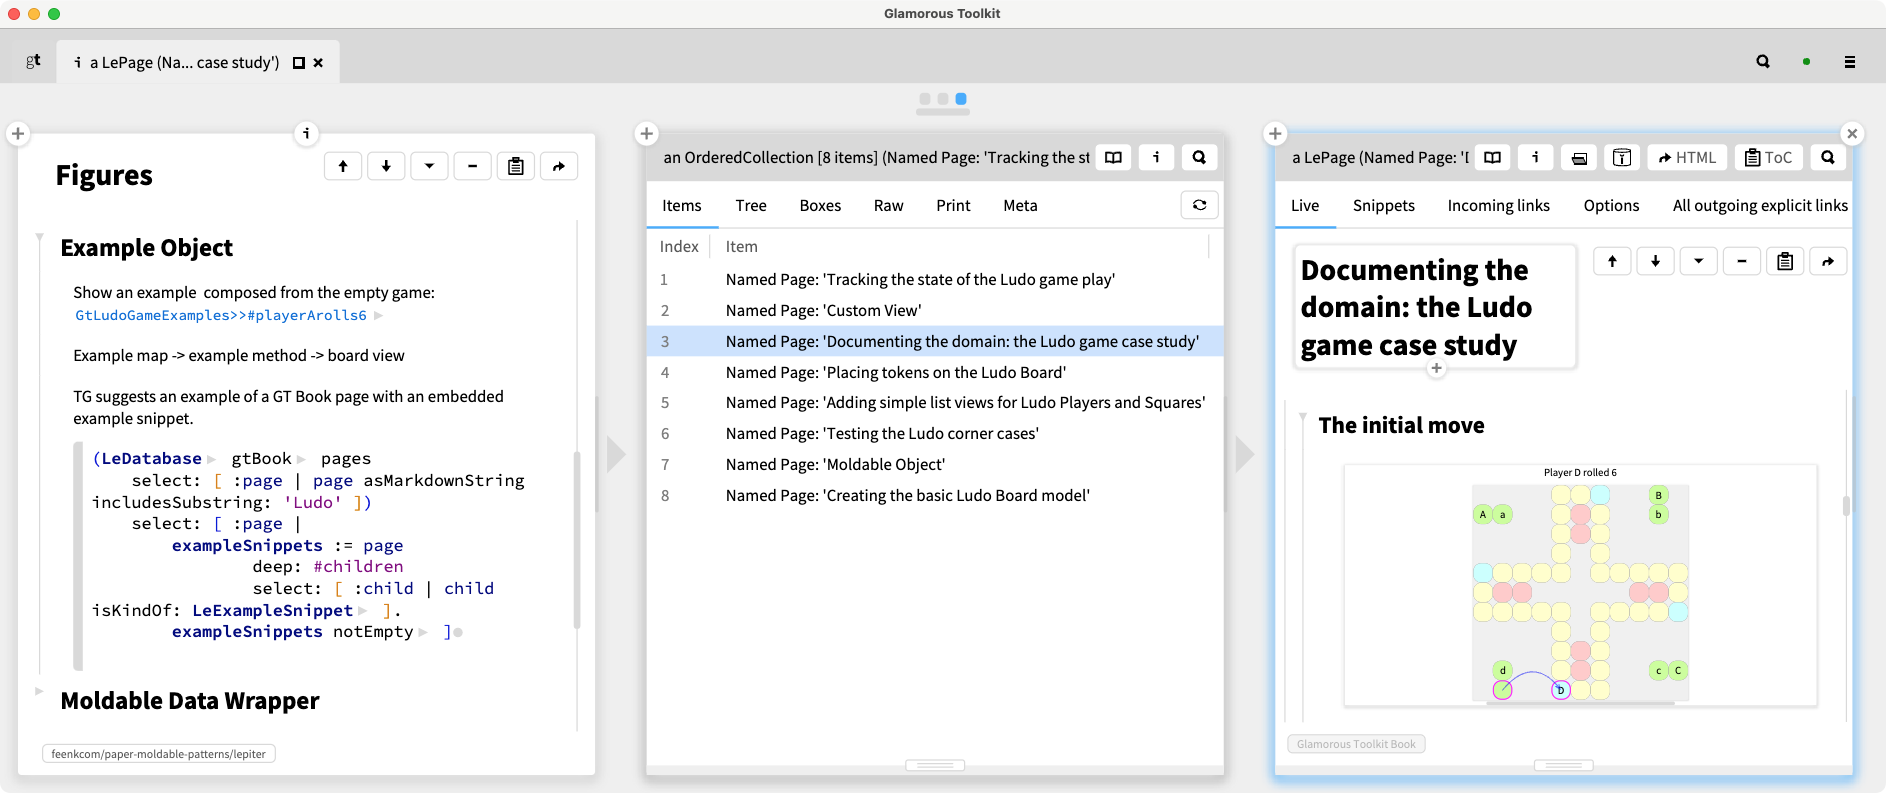
\includegraphics[width=\columnwidth]{throwawayQueryTool}
  \caption{A throwaway analysis to find candidate examples.}
  \label{fig:throwawayQueryTool}
\end{figure}

\eog{Project Diary, I think this is really cool.
It's just not legible in this size.
I wonder if splitting it over to figures to enhance its legibility.}

A throwaway analysis tool should be cheap to implement.
In \autoref{fig:throwawayQueryTool} we see an \emph{ad hoc} query to find Lepiter \pattern{projectDiary} pages that match the string ``\st{Ludo}'' and also contain \pattern{exampleObject} snippets, to illustrate the use of example objects in documentation.

Throwaway analysis tools may appear to be wasteful: they cost development effort that you do not get to reuse.
However, the goal is to optimize the overall development speed.
The alternative to custom tools is manual exploration.
Building a tool, even for just one usage, can outcompete manual exploration by a large margin.
That budget difference can more than make up for the cost of the tool development.

\subsubsection*{Consequences}
By making it cheap to build analysis tools, tool-building becomes an essential part of the development process, rather than a side activity, just as writing tests has become an integral development activity rather than an add-on.

% ===== Conclusion =========================
\section{Conclusion}

The pattern language described here has been mined from several years of experience in applying moldable development to both open- and closed-source projects, using the \GT moldable development platform.
Moldable development makes software systems explainable by making it cheap to add custom tools that support decision making.
In practice, however, this requires a paradigm shift since it leverages live programming to explore domain objects and incrementally mold them.

Although the examples given here have all been drawn from \GT, we believe that they can be applied in any programming environment that offers a minimal level of support for live programming.
The key to supporting moldable development is the pattern \pattern{moldableTool}.
The tools of the environment need to be open to small, custom changes that support decision-making by answering questions about the underlying system under development.
An example of another system that support such changes is Emacs~\cite{Stal81a}, though it was not designed to support moldable development as we describe it.
Once the development environment has been opened up to make its core tools moldable, then moldable development can truly start.

% ===== Acknowledgements =========================
\subsubsection*{Acknowledgements}

We would like to thank Ralf Barkow, Ward Cunningham, Konrad Hinsen, Timo Kehrer and Edward Ocampo-Gooding for their detailed reviews of drafts of this paper.
% Alberto Torres, -- didn't reply

% ===== References =========================
%% The next two lines define the bibliography style to be used, and
%% the bibliography file.
\bibliographystyle{ACM-Reference-Format}
\bibliography{moldablePatterns}

\end{document}
\endinput

% ===== TEMPLATES =========================

\begin{inparaenum}[(i)]
\item
\item
\end{inparaenum}

%: --- CONTINUE HERE
\here

% ----- PATTERN -------------------------
\subsection*{PATTERN}\label{pat:PATTERN}
\subsubsection*{Context}
\subsubsection*{Problem}
\subsubsection*{Forces}
\subsubsection*{Solution}
\subsubsection*{Consequences}
